\documentclass[aps,pre,twocolumn,superscriptaddress]{revtex4-2}

\usepackage[utf8]{inputenc}
\usepackage[T1]{fontenc}
\usepackage{graphicx}
\graphicspath{{../../figures/}}
\usepackage{amsmath,amsthm}
\usepackage{amssymb}
\usepackage{nicefrac}
\usepackage{tikz}
\usepackage{tcolorbox}
\usepackage{hyperref} % hyperref should be loaded late
\usepackage{cleveref}
\usepackage{subcaption}
\usepackage{orcidlink}
\usepackage{booktabs}

%\usetikzlibrary{positioning,arrows.meta,fit,calc}

\begin{document}

% --- Document Information ---
\title{ Supporting Information for:
Plant-wide Bayesian fault diagnosis in recycle processes via simulation-based
inference under multi-loop feedback control
}

\author{Simone Casolo \orcidlink{0000-0003-2945-8931}
}
\email{simone.casolo@cognite.com} 
\affiliation{Cognite AS, Oslo, Norway}

\author{Alexander Johannes Stasik \orcidlink{0000-0003-1646-2472}}
\email{alexander.stasik@sintef.no} 

\affiliation{Department of Data Science, Norwegian University of Life Sciences, \AA s, Norway}
\affiliation{Department for Mathematics and Cybernetics, SINTEF Digital, Oslo, Norway}


\author{Signe Riemer-Sørensen\orcidlink{0000-0002-5308-7651}
}
\affiliation{Department for Mathematics and Cybernetics, SINTEF Digital, Oslo, Norway}

\date{\today}

\maketitle

% =============================================================================
\section*{S1.\; Stochastic Data Generation and Scenario Overview}
\label{sec:si_data_generation}
% =============================================================================

\paragraph{Simulation pipeline.}
Observation windows are generated by integrating the degraded closed-loop model
(Eqs.~(3)--(6) of the main text) with the Euler--Maruyama scheme at a fixed step
of $\Delta t = 0.1$~min.  Two independent noise layers are applied.  \emph{Process
noise} is injected at each integration step as an additive Gaussian increment:
$\boldsymbol{\sigma} = [\sigma_C,\,\sigma_T,\,\sigma_{T_c}] =
[5\times10^{-4}$~mol~L$^{-1}$\,min$^{-1/2}$,\;
$0.1$~K~min$^{-1/2}$,\;$0.1$~K~min$^{-1/2}]$,
consistent with mild process variability at steady state.  \emph{Sensor noise}
is applied post-simulation as a zero-mean Gaussian draw with standard deviation
equal to 0.5\% of each channel's running maximum, representing a typical
industrial-grade sensor specification.

Each replicate is initialised from the nominal closed-loop steady state, computed
by integrating the deterministic ODE to convergence with a high-accuracy adaptive
solver.  Initialising from the steady state removes startup transients and ensures
that the 60-minute window is representative of stationary operation around the
prescribed $(\alpha^*,\beta^*)$ operating point.  The four observable channels
$[C(t),\,T(t),\,T_c(t),\,Q_c(t)]$ are subsampled to a grid of $\Delta t_\mathrm{out}
= 0.5$~min, yielding one $120\times4$ observation matrix per replicate.

\paragraph{Dataset structure.}
The full System~I dataset comprises $8$ scenarios $\times$ $50$ independent
stochastic replicates $= 400$ observation windows.  The eight scenarios
(Table~1 of the main text) span open- and closed-loop configurations and a
range of fault severities; their ground-truth parameters $(\alpha^*,\beta^*)$
are summarised in Table~1 of the main text.  Each replicate
within a scenario shares the same ground-truth $(\alpha^*,\beta^*)$ but was
integrated with an independent random seed, so the 50 replicates per scenario
are exchangeable draws from $p(\mathbf{x}\mid\alpha^*,\beta^*)$ at that
operating point.

\paragraph{Scenario trajectories.}
Figure~\ref{fig:si_scenarios} shows six representative replicates per closed-loop
scenario across all four observable channels.  The bold black trace is the
per-scenario replicate mean.

Several features are immediately apparent.  First, the reactor temperature $T$
is tightly regulated near the setpoint $T_\mathrm{sp} = 312.5$~K in all
non-saturating scenarios: the PI controller maintains the same temperature
profile regardless of whether the jacket is fouled (Sc\,2) or the catalyst
is decaying (Sc\,3), confirming the closed-loop masking mechanism discussed in
Section~2.2 of the main text.  Second, the coolant flow $Q_c$ shows
qualitatively distinct behaviour across scenarios: jacket fouling (Sc\,2) drives
$Q_c$ to $\approx 210$~L~min$^{-1}$, while catalyst decay (Sc\,3) lowers it
to $\approx 50$~L~min$^{-1}$, and severe fouling (Sc\,5) saturates the valve
at $Q_{c,\max} = 400$~L~min$^{-1}$.  Third, the concentration channel $C$
shifts distinctly between scenarios with different $\alpha^*$: catalyst decay
(Sc\,3, $\alpha^*=0.70$) raises $C_\mathrm{ss}$ from $\approx 0.018$ to
$\approx 0.026$~mol~L$^{-1}$, while jacket fouling (Sc\,2) produces a modest
downward shift attributable to the residual thermal coupling through $T_c$.
The sensor-drift scenario (Sc\,7, $\delta_T = +2$~K) is indistinguishable from
Sc\,1 in the $C$ and $T_c$ channels but shows a systematic upward offset in
the $T$ channel, motivating the four-dimensional
$(\alpha,\beta,\delta_T,\delta_{C_i})$ extension explored in future work.

% ------------------------------------------------------------------
\begin{figure*}[htbp]
  \centering
  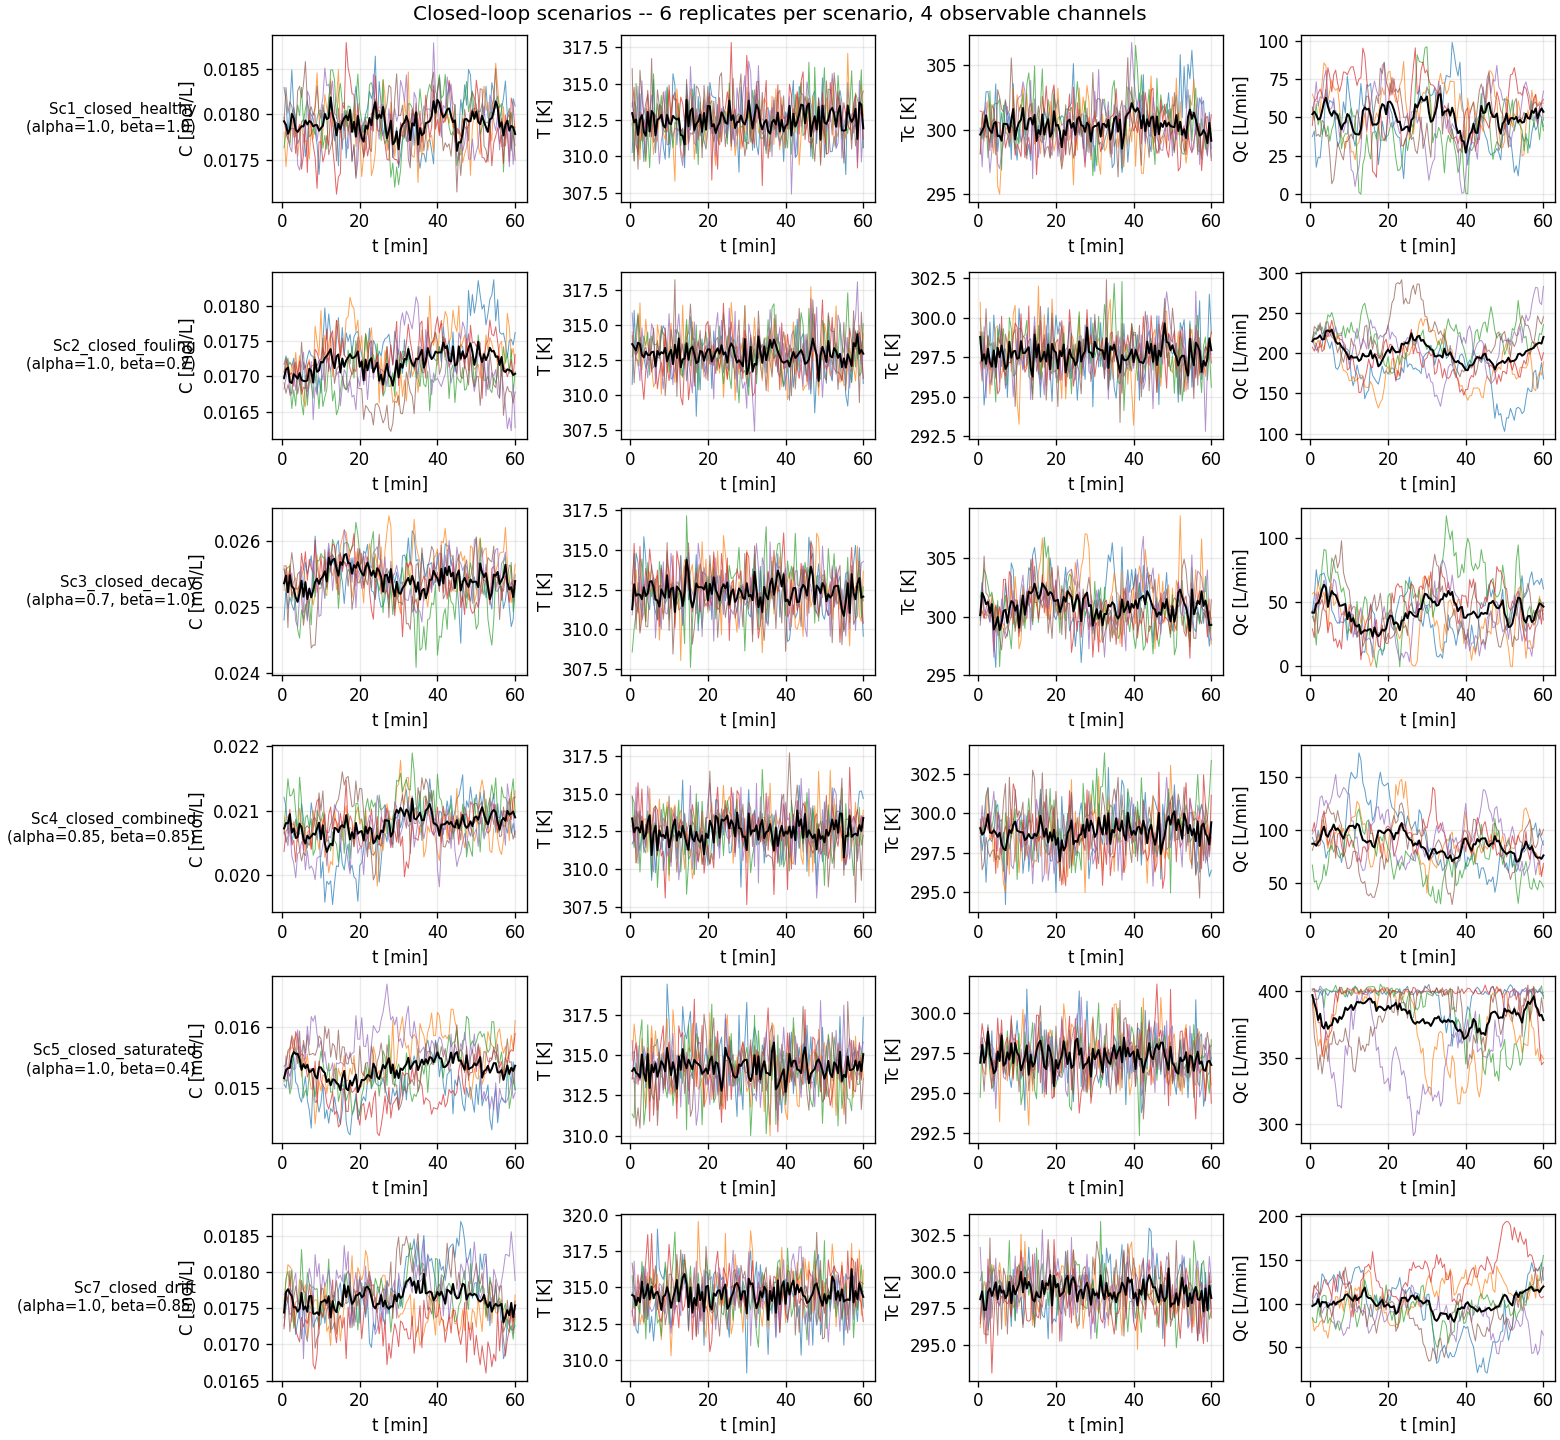
\includegraphics[width=\linewidth]{02_scenarios_overview}
  \caption{Representative observation windows for the six closed-loop fault
    scenarios (Sc\,1--5, Sc\,7).  Each row corresponds to one scenario
    (scenario name and ground-truth $(\alpha^*,\beta^*)$ shown on the left);
    columns show the four observable channels
    $[C,\,T,\,T_c,\,Q_c]$ over the 60-minute window.
    Coloured traces: six individual stochastic replicates.
    Bold black trace: replicate mean.
    The reactor temperature $T$ (second column) is regulated near
    $T_\mathrm{sp} = 312.5$~K across all scenarios; the fault signal is
    encoded primarily in $Q_c$ (fourth column) and $C$ (first column),
    consistent with the Fisher-information analysis in Section~4.3.1 of
    the main text.}
  \label{fig:si_scenarios}
\end{figure*}
% ------------------------------------------------------------------

% ------------------------------------------------------------------
\begin{figure*}[htbp]
  \centering
  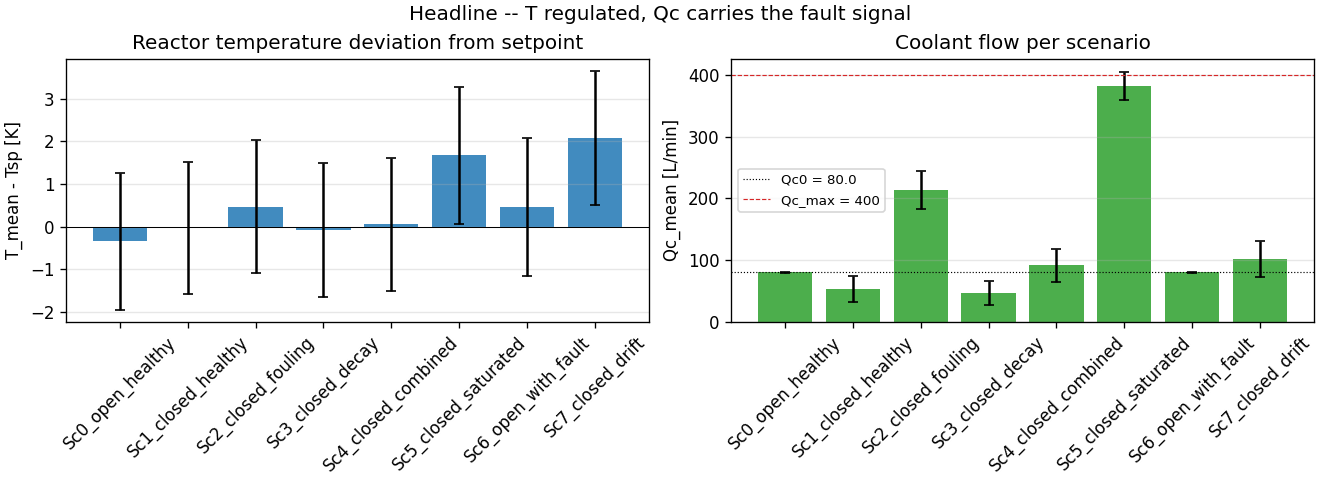
\includegraphics[width=0.90\linewidth]{02_headline_summary}
  \caption{Headline summary of the closed-loop masking effect across all
    eight scenarios (50 stochastic replicates each, 60-min windows).
    \textit{Left:} Mean reactor temperature deviation from setpoint
    $\bar{T} - T_\mathrm{sp}$ with $\pm1\sigma$ error bars.  Under
    non-saturating PI control, $\bar{T} - T_\mathrm{sp} \approx 0$
    for all closed-loop scenarios regardless of fault severity.
    \textit{Right:} Mean coolant flow rate $\bar{Q}_c$ per scenario.
    Jacket fouling (Sc\,2) raises $\bar{Q}_c$ to $\approx 210$~L~min$^{-1}$;
    catalyst decay (Sc\,3) reduces it to $\approx 50$~L~min$^{-1}$;
    severe fouling (Sc\,5) saturates the valve at $Q_{c,\max}=400$~L~min$^{-1}$.
    The fault signal lives entirely in the actuator output, not in the
    regulated reactor temperature.}
  \label{fig:headline_summary}
\end{figure*}
% ------------------------------------------------------------------

% =============================================================================
\section*{S2.\; Prior Predictive Check}
\label{sec:si_prior_predictive}
% =============================================================================

A necessary condition for valid amortised inference is that the prior-predictive
distribution --- the distribution of summary statistics produced by prior draws ---
covers the evaluation observations.  To verify this, we drew 500 parameter vectors
$\boldsymbol{\theta}=(\alpha,\beta)$ from the uniform prior~$\mathcal{U}([0.4,1.2]^2)$
and simulated each through the stochastic closed-loop model to obtain synthetic
60-minute observation windows.  For every feature in the 29-D summary vector, the
$[2.5\%,\,97.5\%]$ interval of the prior-predictive distribution was compared against
the observed values from all six closed-loop evaluation scenarios (Sc\,1--5, Sc\,7).
At least 80\% of the observed values per feature fall inside this interval, confirming
that the simulator faithfully spans the evaluation regime.

Figure~\ref{fig:si_simulator_sanity} illustrates the check for four representative
features, including the two physics-informed proxies that carry most of the
identifying information about $(\alpha,\beta)$ (see Section~3.1 of the main text).
The observed scenario means (vertical markers) are well contained within the
prior-predictive histograms for every feature shown, with no scenario lying
systematically outside the prior envelope.

% ------------------------------------------------------------------
\begin{figure*}[htbp]
  \centering
  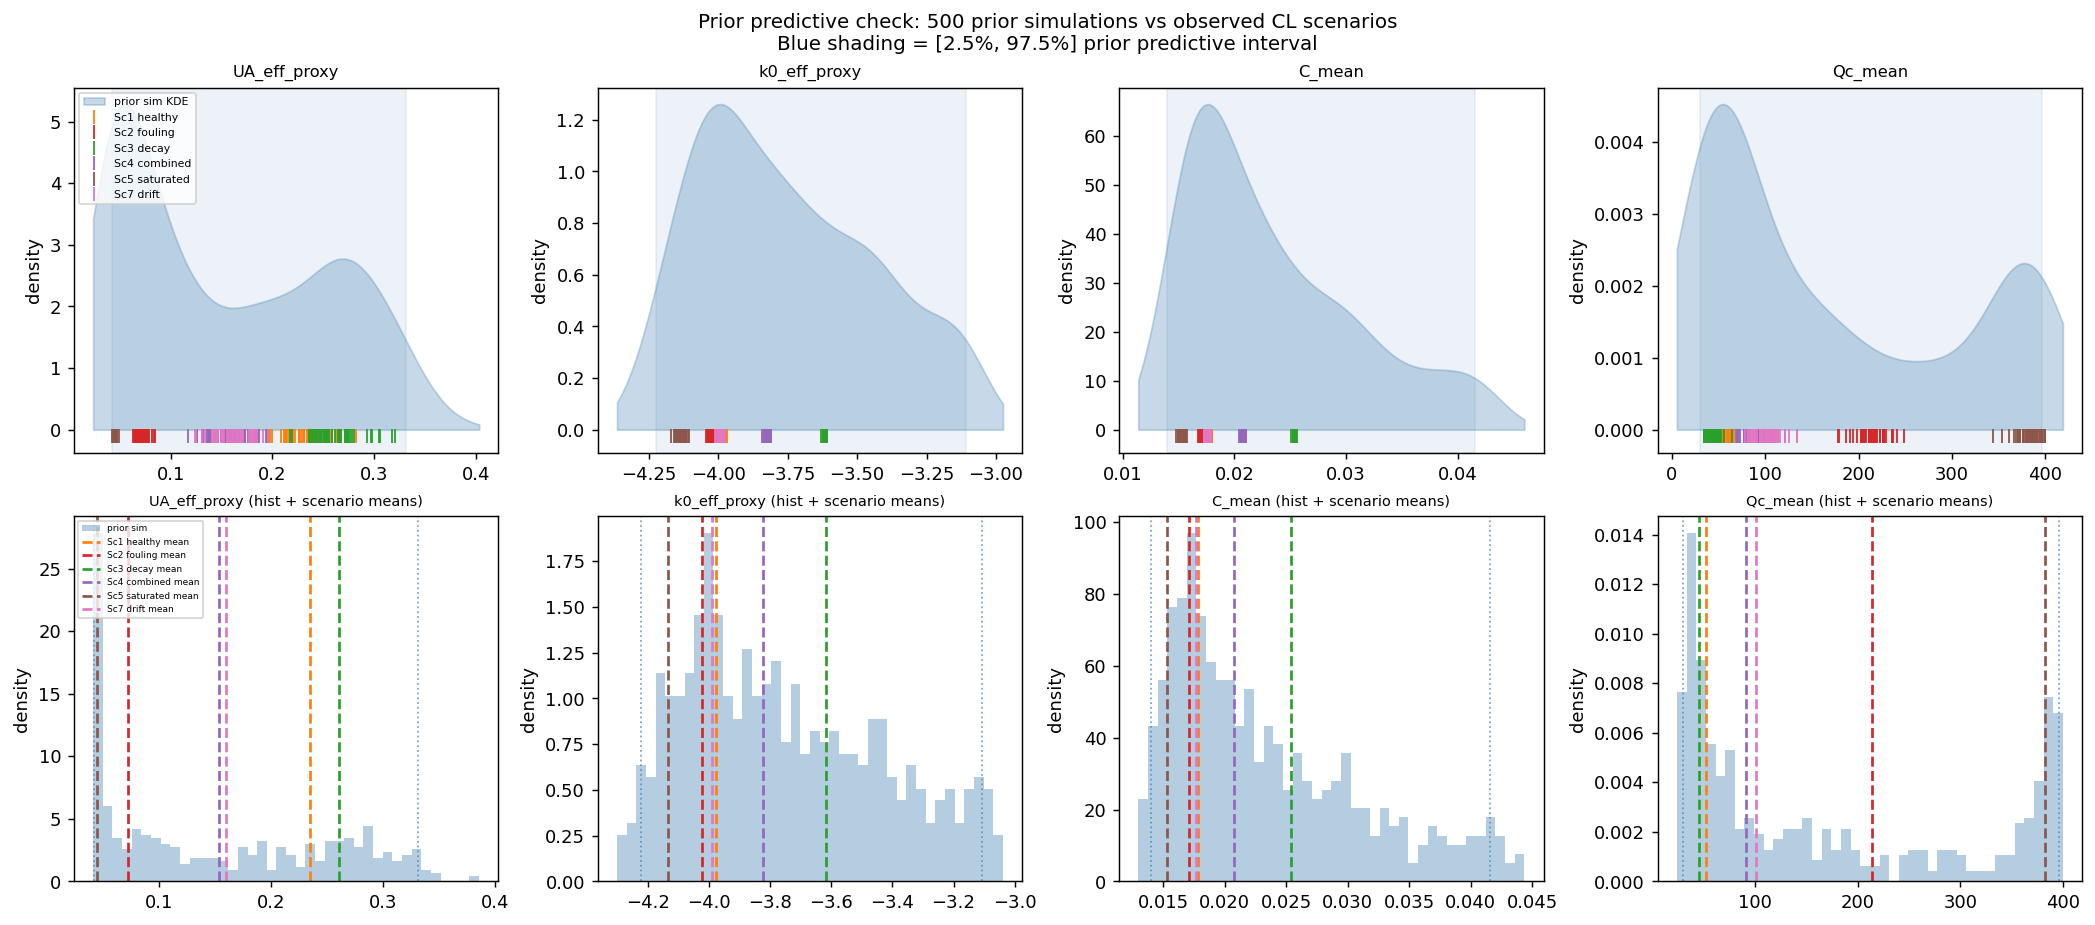
\includegraphics[width=0.97\linewidth]{04_simulator_sanity}
  \caption{Prior predictive check ($N=500$ prior draws) for four key summary
    features: $s_{U\!A}$, $s_{k_0}$, $\bar{C}$, and $\bar{Q}_c$.
    \textit{Top row:} kernel density estimates of the prior-predictive
    distribution (blue fill) with observed values from each closed-loop scenario
    overlaid as tick marks.
    \textit{Bottom row:} histogram of prior-predictive values with per-scenario
    means marked as vertical lines.
    All scenario observations fall within the prior-predictive envelope,
    confirming that the simulator covers the operating regime of the
    evaluation set.}
  \label{fig:si_simulator_sanity}
\end{figure*}
% ------------------------------------------------------------------

% =============================================================================
\section*{S3.\; Training Budget Sensitivity}
\label{sec:si_sensitivity}
% =============================================================================

To confirm that the choice of $n_\mathrm{sim}=10{,}000$ training simulations is
sufficient, we trained three posteriors using MAF density estimators at budgets
of $1{,}000$, $5{,}000$, and $10{,}000$ prior draws and evaluated each on the healthy
scenario (Sc\,1, $\alpha^*=\beta^*=1.0$) and the jacket-fouling scenario
(Sc\,2, $\beta^*=0.70$).

All three budgets achieve 90\% credible-interval coverage of the true parameters on
Sc\,1.  For Sc\,2, the posterior mean of $\beta$ shifts monotonically from
$\hat{\beta}=0.680$ at $n_\mathrm{sim}=1{,}000$ to $\hat{\beta}=0.618$ at
$n_\mathrm{sim}=10{,}000$, while 90\% CI coverage is attained at all three budgets.
Increasing the budget beyond 10,000 produced no measurable improvement in the
simulation-based calibration metrics (Section~S6), motivating the choice of
$n_\mathrm{sim}=10{,}000$ for the production NSF posterior.

The persistent $\hat{\beta}$ bias observed across all three budgets is not a training
artefact: it is the structural closed-loop masking effect characterised analytically
in Section~4.3 of the main text and confirmed by four independent inference methods.

% ------------------------------------------------------------------
\begin{figure*}[htbp]
  \centering
  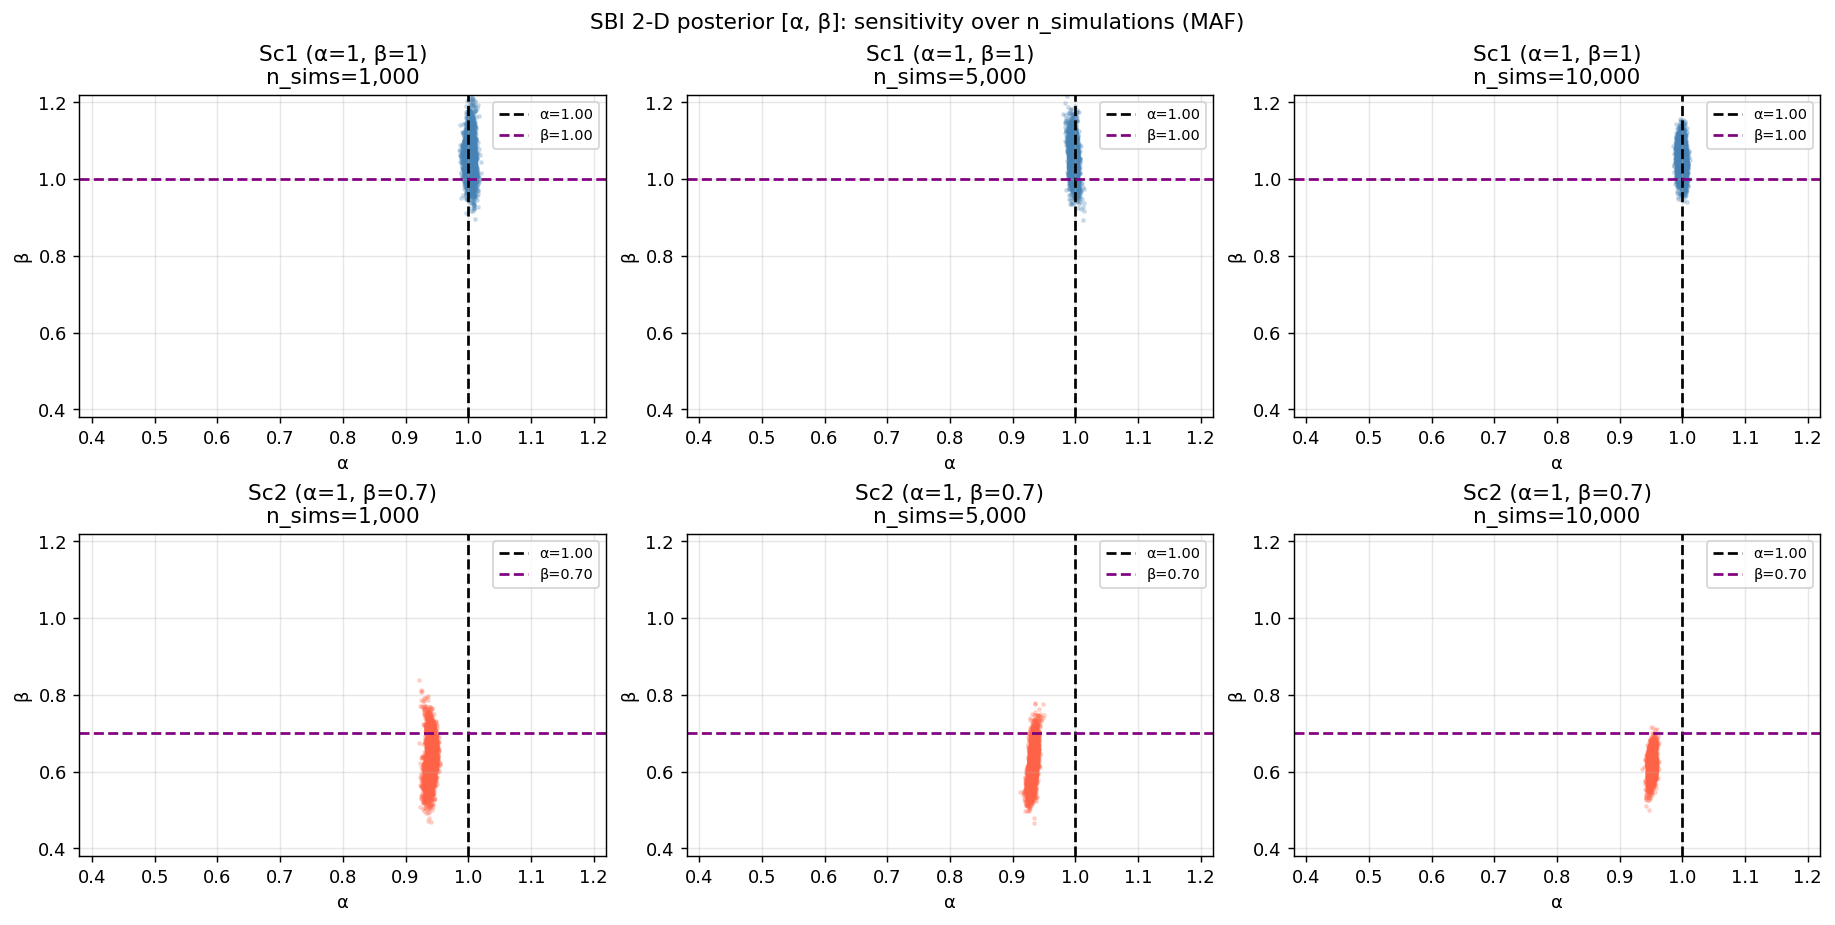
\includegraphics[width=0.95\linewidth]{04_sensitivity_scatter}
  \caption{Training budget sensitivity: 2-D posterior scatter plots $[\alpha,\beta]$
    for Sc\,1 (healthy, top row) and Sc\,2 (jacket fouling, bottom row) at three
    simulation budgets (MAF estimator).  Dashed lines mark the true parameter
    values.  All three budgets achieve 90\% credible-interval coverage; the posterior
    concentrates monotonically with $n_\mathrm{sim}$, with no change in the
    systematic $\beta$ underestimation that characterises all inference methods on
    this closed-loop dataset.}
  \label{fig:si_sensitivity}
\end{figure*}
% ------------------------------------------------------------------

\section{summary statistics}

\paragraph{Group~1 --- Per-channel base statistics (20 features).}
For each of the four observable channels $[C, T, T_c, Q_c]$, five
scalar statistics are computed over the full 60-minute window: the
arithmetic mean, standard deviation, ordinary-least-squares slope,
minimum, and maximum.  These 20 features capture the level, variability,
trend, and range of each signal and form the baseline subset against
which the additional groups are evaluated.

\paragraph{Group~2 --- Final-window means (4 features).}
The arithmetic mean of each channel over the final 25\% of the observation
window (minutes 45--60) provides an estimate of the current
quasi-steady-state operating point, less contaminated by fault-onset
transients than the whole-window mean.  Under stationary closed-loop
operation these four values converge to the steady-state measurements
$C_\mathrm{ss}$, $T_\mathrm{ss}$, $T_{c,\mathrm{ss}}$, and
$Q_{c,\mathrm{ss}}$.

\paragraph{Group~3 --- Control aggregates (3 features).}
Three aggregates quantify the operational burden placed on the PI
controller during the observation window:
%
\begin{itemize}
  \item $\int_0^{60}\lvert T(t)-T_\mathrm{sp}\rvert\,\mathrm{d}t$: the
    time-integrated absolute temperature error, which increases whenever
    the controller is unable to maintain the setpoint, most prominently
    during the actuator-saturation regime of Sc\,5.
  \item $f_\mathrm{sat,\,low}$: the fraction of time steps at which
    $Q_c = Q_{c,\min} = 0$~L~min$^{-1}$, indicating fully-closed valve
    saturation.
  \item $f_\mathrm{sat,\,high}$: the fraction of time steps at which
    $Q_c = Q_{c,\max} = 400$~L~min$^{-1}$, indicating fully-open
    saturation.
\end{itemize}
%
All three aggregates equal zero under healthy, non-saturating closed-loop
operation and become the dominant diagnostic features in the degraded
regimes where the per-channel statistics carry reduced discriminating power.

\paragraph{Group~4 --- Physics-informed proxies (2 features).}
Two features are derived by algebraic inversion of the closed-loop
steady-state balance equations, making them direct proxies for the
identifiable parameter products $\beta\!\cdot\!U\!A$ and
$\alpha\!\cdot\!k_0$:
%
\begin{align}
  s_{U\!A} &= \frac{\bar{T}-\bar{T}_c}{\bar{Q}_c},
  \label{eq:ua_proxy}\\[4pt]
  s_{k_0} &= \ln\!\left(\frac{\bar{C}}{C_i - \bar{C}}\right),
  \label{eq:k0_proxy}
\end{align}
%
where $\bar{(\cdot)}$ denotes the whole-window mean of the respective
channel.  Under non-saturating PI control at steady state,
$s_{U\!A}\propto(\beta\!\cdot\!U\!A)^{-1}$ follows from the jacket energy
balance, and $s_{k_0}\propto(\alpha\!\cdot\!k_0)^{-1}$ follows from the
component balance at fixed conversion.  Used alone, these two features
achieve 98.3\% cross-validated Linear Discriminant Analysis (LDA) \citep{Zhou2021}
accuracy on the eight-scenario dataset, confirming that they encode nearly all of the identifiable
information about $(\alpha,\beta)$ accessible from stationary, noise-free
steady-state observations.  Figure~\ref{fig:physics_scatter} illustrates
this separation directly: all eight scenarios occupy well-separated,
compact clusters in the $(s_{U\!A},\,s_{k_0})$ plane.


% =============================================================================
\section*{S4.\; PCA Manifold of Summary Statistics}
\label{sec:si_pca}
% =============================================================================

To complement the physics-proxy scatter plot shown in the main text, Figure~%
\ref{fig:si_pca} shows the principal component analysis (PCA) projection of the
standardised 29-D summary vectors across all 400 observation windows (8 scenarios,
50 replicates each).

All eight scenarios occupy visually distinct regions in the PC1--PC2 projection,
which together account for 57.7\% of the total variance.  The severe-fouling scenario
(Sc\,5) separates primarily along PC1, driven by the saturation-fraction features that
are identically zero in all other scenarios.  The open-loop scenarios (Sc\,0, Sc\,6;
squares) are resolved from their closed-loop counterparts in the PC3--PC4 projection,
where the standard deviation and slope of $Q_c$ provide the distinguishing signal.

This global separability confirms that the 29-D vector encodes adequate information
for all eight scenarios, including regimes --- such as valve saturation and open-loop
operation --- where the two physics-proxy features $s_{U\!A}$ and $s_{k_0}$ lose
discriminating power.

% ------------------------------------------------------------------
\begin{figure*}[htbp]
  \centering
  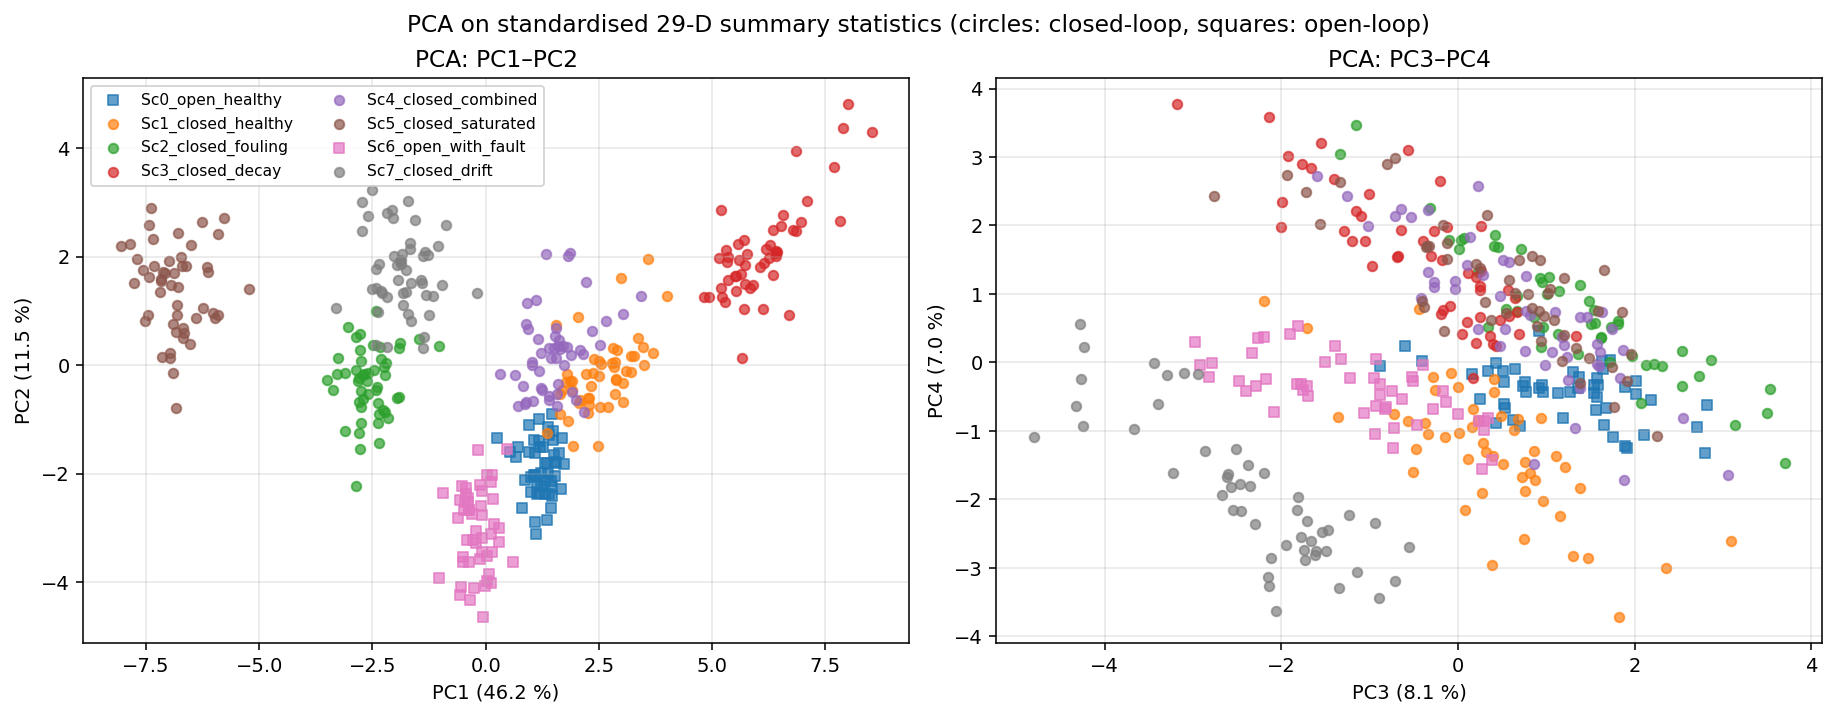
\includegraphics[width=0.92\linewidth]{03_pca}
  \caption{PCA of the standardised 29-D summary-statistic vectors (400 windows,
    8 scenarios).  Circles: closed-loop replicates; squares: open-loop replicates
    (Sc\,0, Sc\,6).
    \textit{Left:} PC1--PC2 projection (46.2\% + 11.5\% variance explained).
    \textit{Right:} PC3--PC4 projection further resolves the open-loop scenarios
    from their closed-loop counterparts.}
  \label{fig:si_pca}
\end{figure*}
% ------------------------------------------------------------------


Each 2-hour observation window $\mathbf{x}\in\mathbb{R}^{120\times9}$ 
is compressed to a 66-dimensional 
summary-statistic vector prior to passing it to the neural density
estimator.  The feature groups follow the same four-category structure as System~I
(Section~\ref{sec:summary_stats}): per-channel base statistics, final-window means,
control aggregates, and physics-informed proxies.  Complete feature definitions and
a per-parameter mutual-information ranking are provided in Table~S3 of the Supporting
Information (Section~S9).

Figure~\ref{fig:wu_pca} shows the PCA projection of the standardised 66-D
feature vectors computed from all 420 (noise-free) observation windows (14 scenarios,
30 replicates each).  The reactor-fault scenarios (W2--W6, W11) and the column-fault
scenarios (W7, W9) occupy largely distinct regions of the PC1--PC2 plane, confirming
that the 66-D feature set carries adequate scenario-separating information for most
fault types; the snowball-tipping-point scenario (W4, $\alpha = 0.58$) is an outlier
along PC1, reflecting the nonlinear amplification of the recycle load near the
instability boundary.  Training hyperparameters and posterior calibration results are
given in Section~S7 and S9 of the Supporting Information.

% ------------------------------------------------------------------
\begin{figure}[htbp]
  \centering
  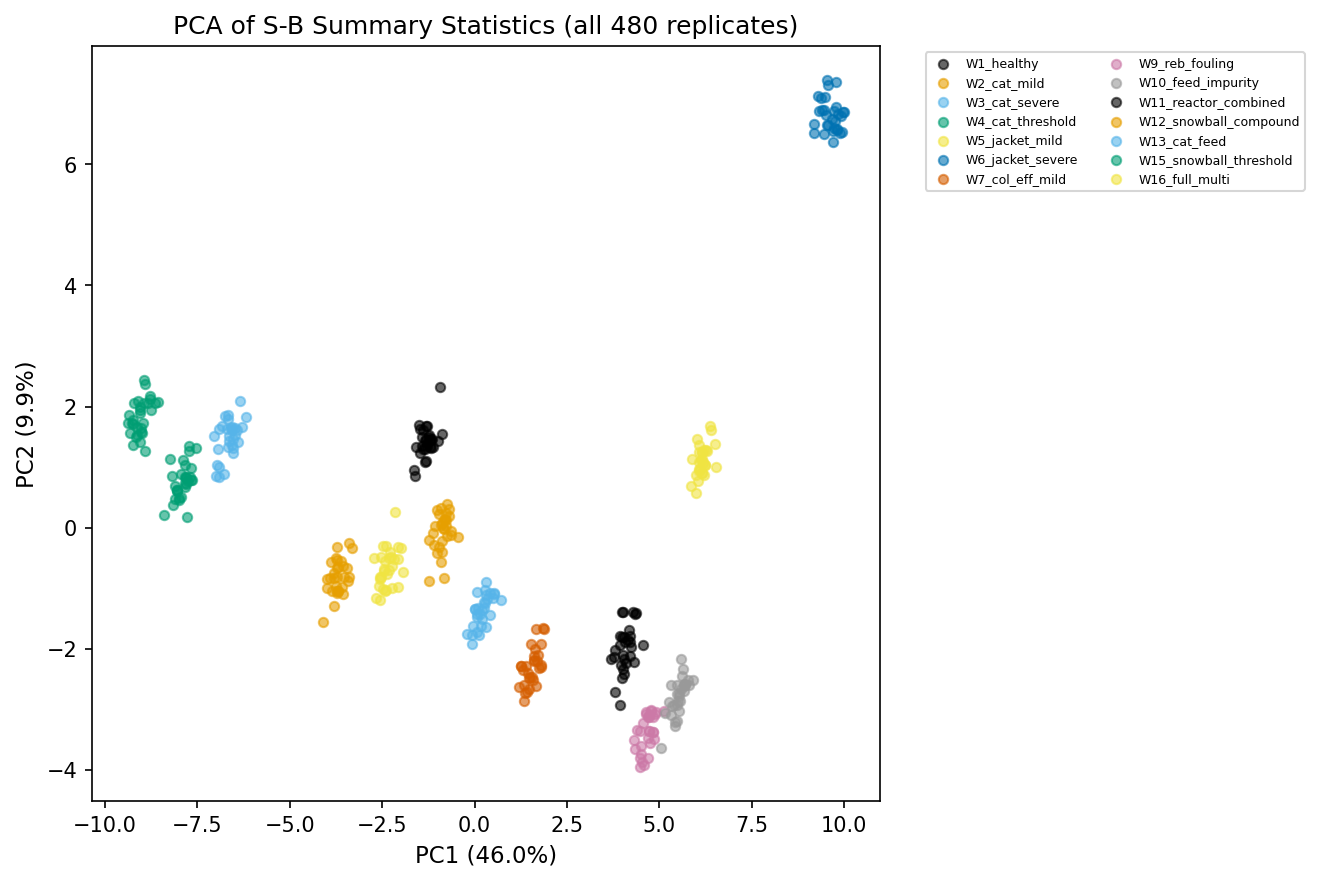
\includegraphics[width=0.97\linewidth]{nb23_pca_sb}
  \caption{PCA of the standardised 66-D summary-statistic vectors
    (420 windows, 14 scenarios). 
    PC1--PC2 projection; reactor-fault and column-fault
    scenario clusters are largely separable.  The near-snowball scenario
    W4 ($\alpha = 0.58$) projects as an outlier along PC1 due to the
    strongly amplified recycle load.}
  \label{fig:wu_pca}
\end{figure}
% ------------------------------------------------------------------




% =============================================================================
\section*{S5.\; Complete Summary-Statistic Definitions and Feature Ablation}
\label{sec:si_features}
% =============================================================================

Table~\ref{tab:si_summary_stats} lists all 29 features that form the summary-statistic
vector $\mathbf{s}\in\mathbb{R}^{29}$ used throughout this work.  The four groups
correspond to those described in Section~3.1 of the main text.

Table~\ref{tab:si_feature_ablation} reports five-fold stratified cross-validated
LDA classification accuracy for seven feature subsets on the 400-window
System~I dataset.  The physics-2 subset (Group~4, two features) alone achieves
98.3\% accuracy, confirming that the steady-state proxy features encode nearly
all scenario-separating information.  The remaining 27 features are necessary
not to improve classification accuracy --- which saturates at 100\% with as few
as four final-window means --- but to correctly quantify posterior uncertainty
under noise, transients, and actuator saturation.  This distinction between
classification accuracy and posterior calibration is central to the argument of
the main text: the 29-D vector is chosen to provide accurate full posterior
distributions, not merely correct fault labels.

Beyond the two-feature theoretical minimum, four practical effects require
additional features: sensor noise amplifies in the ratio $s_{U\!A}$ at moderate
$Q_c$ values, making it preferable to supply the three component channels
separately; slope and final-window features carry transient information during
fault onset; the saturation-fraction features take over from $s_{U\!A}$ when
the valve is fully open (Sc\,5); and the standard deviation of $Q_c$ distinguishes
open-loop windows (constant $Q_c$) from closed-loop ones.

% ------------------------------------------------------------------
\begin{table*}[htbp]
\centering
\caption{Complete summary-statistic vector for System~I: 29 features in four
  groups.  $\bar{(\cdot)}$ = whole-window mean; $(\cdot)_f$ = final-25\%
  window mean; channel indices $[C,T,T_c,Q_c]$.}
\label{tab:si_summary_stats}
\small
\begin{tabular}{clrc}
\toprule
Group & Features & Count & Physical motivation \\
\midrule
1 & mean, std, slope, min, max $\times$ $[C,T,T_c,Q_c]$ & 20 & Level, variability, trend \\
2 & $C_f$, $T_f$, $T_{c,f}$, $Q_{c,f}$                 & 4  & Quasi-steady-state estimate \\
3 & $\int\lvert T-T_\mathrm{sp}\rvert\,\mathrm{d}t$,
    $f_\mathrm{sat,\,low}$, $f_\mathrm{sat,\,high}$    & 3  & Controller load / saturation \\
4 & $s_{U\!A}$,\; $s_{k_0}$                             & 2  & Physics-informed proxies \\
\midrule
Total &                                                   & 29 & \\
\bottomrule
\end{tabular}
\end{table*}
% ------------------------------------------------------------------

% ------------------------------------------------------------------
\begin{table}[htbp]
\centering
\caption{Feature-subset ablation: five-fold stratified cross-validated LDA
  accuracy on the 400-window System~I dataset (8 scenarios, 50 replicates each).
  MI = mutual information with scenario label.  The saturation of accuracy at
  100\% for several subsets shows that classification difficulty does not
  determine the choice of feature set; posterior calibration does.}
\label{tab:si_feature_ablation}
\small
\begin{tabular}{lrr}
\toprule
Feature subset                    & $n$ features & CV accuracy \\
\midrule
Full 29-D vector                  & 29  & 1.000 \\
Top-10 MI shortlist               & 10  & 0.991 \\
Top-5 MI shortlist                & 5   & 0.979 \\
Group~4 (physics-2)               & 2   & 0.983 \\
Group~3 (control aggregates)      & 3   & 0.800 \\
Group~2 (final-window means)      & 4   & 1.000 \\
Group~1 (per-channel base)        & 20  & 0.998 \\
\bottomrule
\end{tabular}
\end{table}
% ------------------------------------------------------------------

% =============================================================================
\section*{S6.\; Posterior Calibration: Simulation-Based Calibration Protocol
  and Results}
\label{sec:si_sbc}
% =============================================================================

\paragraph{Protocol.}
Posterior calibration is assessed using simulation-based calibration~%
\citep{Talts2018}.  In SBC, $N_\mathrm{SBC}$ parameter vectors
$\boldsymbol{\theta}^{(i)}$ are drawn independently from the prior; for each draw
a synthetic observation $\mathbf{x}^{(i)}$ is simulated and the posterior is sampled
to obtain $L$ approximate draws $\{\tilde{\boldsymbol{\theta}}^{(i)}_\ell\}_{\ell=1}^L$.
The rank of the true parameter among the posterior draws,
%
\begin{equation}
  r^{(i)}_j
  = \sum_{\ell=1}^{L}
    \mathbf{1}\!\left\{\tilde{\theta}^{(i)}_{\ell,j} < \theta^{(i)}_j\right\},
\end{equation}
%
is recorded for each marginal $j\in\{\alpha,\beta\}$.  A well-calibrated posterior
yields rank statistics that are uniformly distributed on $\{0,1,\ldots,L\}$ across
all $N_\mathrm{SBC}$ test cases.  Uniformity is assessed via the
Kolmogorov--Smirnov (KS) test and the two-sample classifier score
(C2ST;~\citealt{LopezPaz2017}): a KS $p$-value above $0.05$ indicates that
uniformity cannot be rejected at the 5\% level; a C2ST score below $0.52$ indicates
that the rank distribution is indistinguishable from uniform by a trained binary
classifier~\citep{TejeroCantero2020}.  We use $N_\mathrm{SBC}=500$ test cases and
$L=1{,}000$ posterior draws per case.

\paragraph{Results.}
The KS $p$-values for the production NSF posterior are $0.016$ ($\alpha$) and
$0.014$ ($\beta$), formally rejecting rank uniformity at the 5\% level for both
marginals (Figure~\ref{fig:si_sbc_ranks}).  The C2ST scores are $0.52$ ($\alpha$)
and $0.53$ ($\beta$), both near the uninformative baseline of 0.5.

\paragraph{Interpretation.}
The combination of $p < 0.05$ on the KS test with C2ST $\approx 0.5$ is the
diagnostic signature of a structural information deficit rather than a failure of the
density estimator.  The KS test rejects uniformity because the rank distribution is
systematically compressed toward low values for $\beta$: the PI controller enforces
$T = T_\mathrm{sp}$, removing the temperature channel's contribution to $I_{\beta\beta}$
and producing a posterior that concentrates below the true $\beta$.  The C2ST score
remaining near 0.5 confirms that this compression is subtle and the estimator is
performing correctly given the information in the data.  A miscalibration arising
from a training deficiency --- insufficient simulations, architecture mismatch, or
a distributional gap between training and evaluation --- would instead produce both
a low KS $p$-value \emph{and} a C2ST score substantially above 0.5.  The fact that
neither C2ST score exceeds 0.53 therefore supports the interpretation that the
$n_\mathrm{sim}=10{,}000$ production posterior is well-trained and that the
miscalibration is irreducible from closed-loop data, consistent with the Cram\'er-Rao
argument and the embedding-net irreducibility experiment in Section~4.3.3 of the
main text.

% ------------------------------------------------------------------
\begin{figure}[htbp]
  \centering
  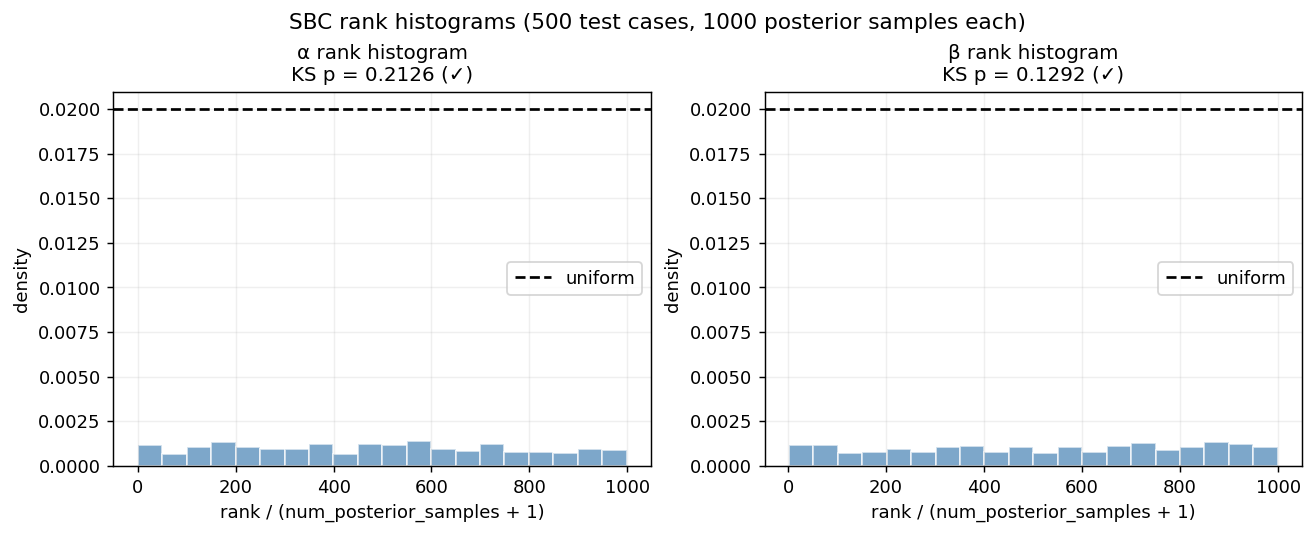
\includegraphics[width=0.97\linewidth]{04_sbc_ranks}
  \caption{SBC rank histograms for the production NSF posterior
    ($N_\mathrm{SBC}=500$ test cases, $L=1{,}000$ posterior draws each).
    Dashed line: expected uniform density.  Both marginals are compressed toward
    low ranks (KS $p=0.016$ for $\alpha$, $p=0.014$ for $\beta$), reflecting the
    systematic downward shift of the $\beta$ posterior caused by the PI controller's
    suppression of the temperature information channel.  The C2ST scores of 0.52
    and 0.53 confirm the miscalibration is subtle and consistent with a structural
    Fisher-information deficit, not a training deficiency.}
  \label{fig:si_sbc_ranks}
\end{figure}
% ------------------------------------------------------------------

% =============================================================================
\section*{S7.\; System II: Fault Scenarios and Data-Generation Details}
\label{sec:si_wu_system}
% =============================================================================

\subsection*{S7.1 Nominal parameter values}

\begin{figure}[htbp]
  \centering
  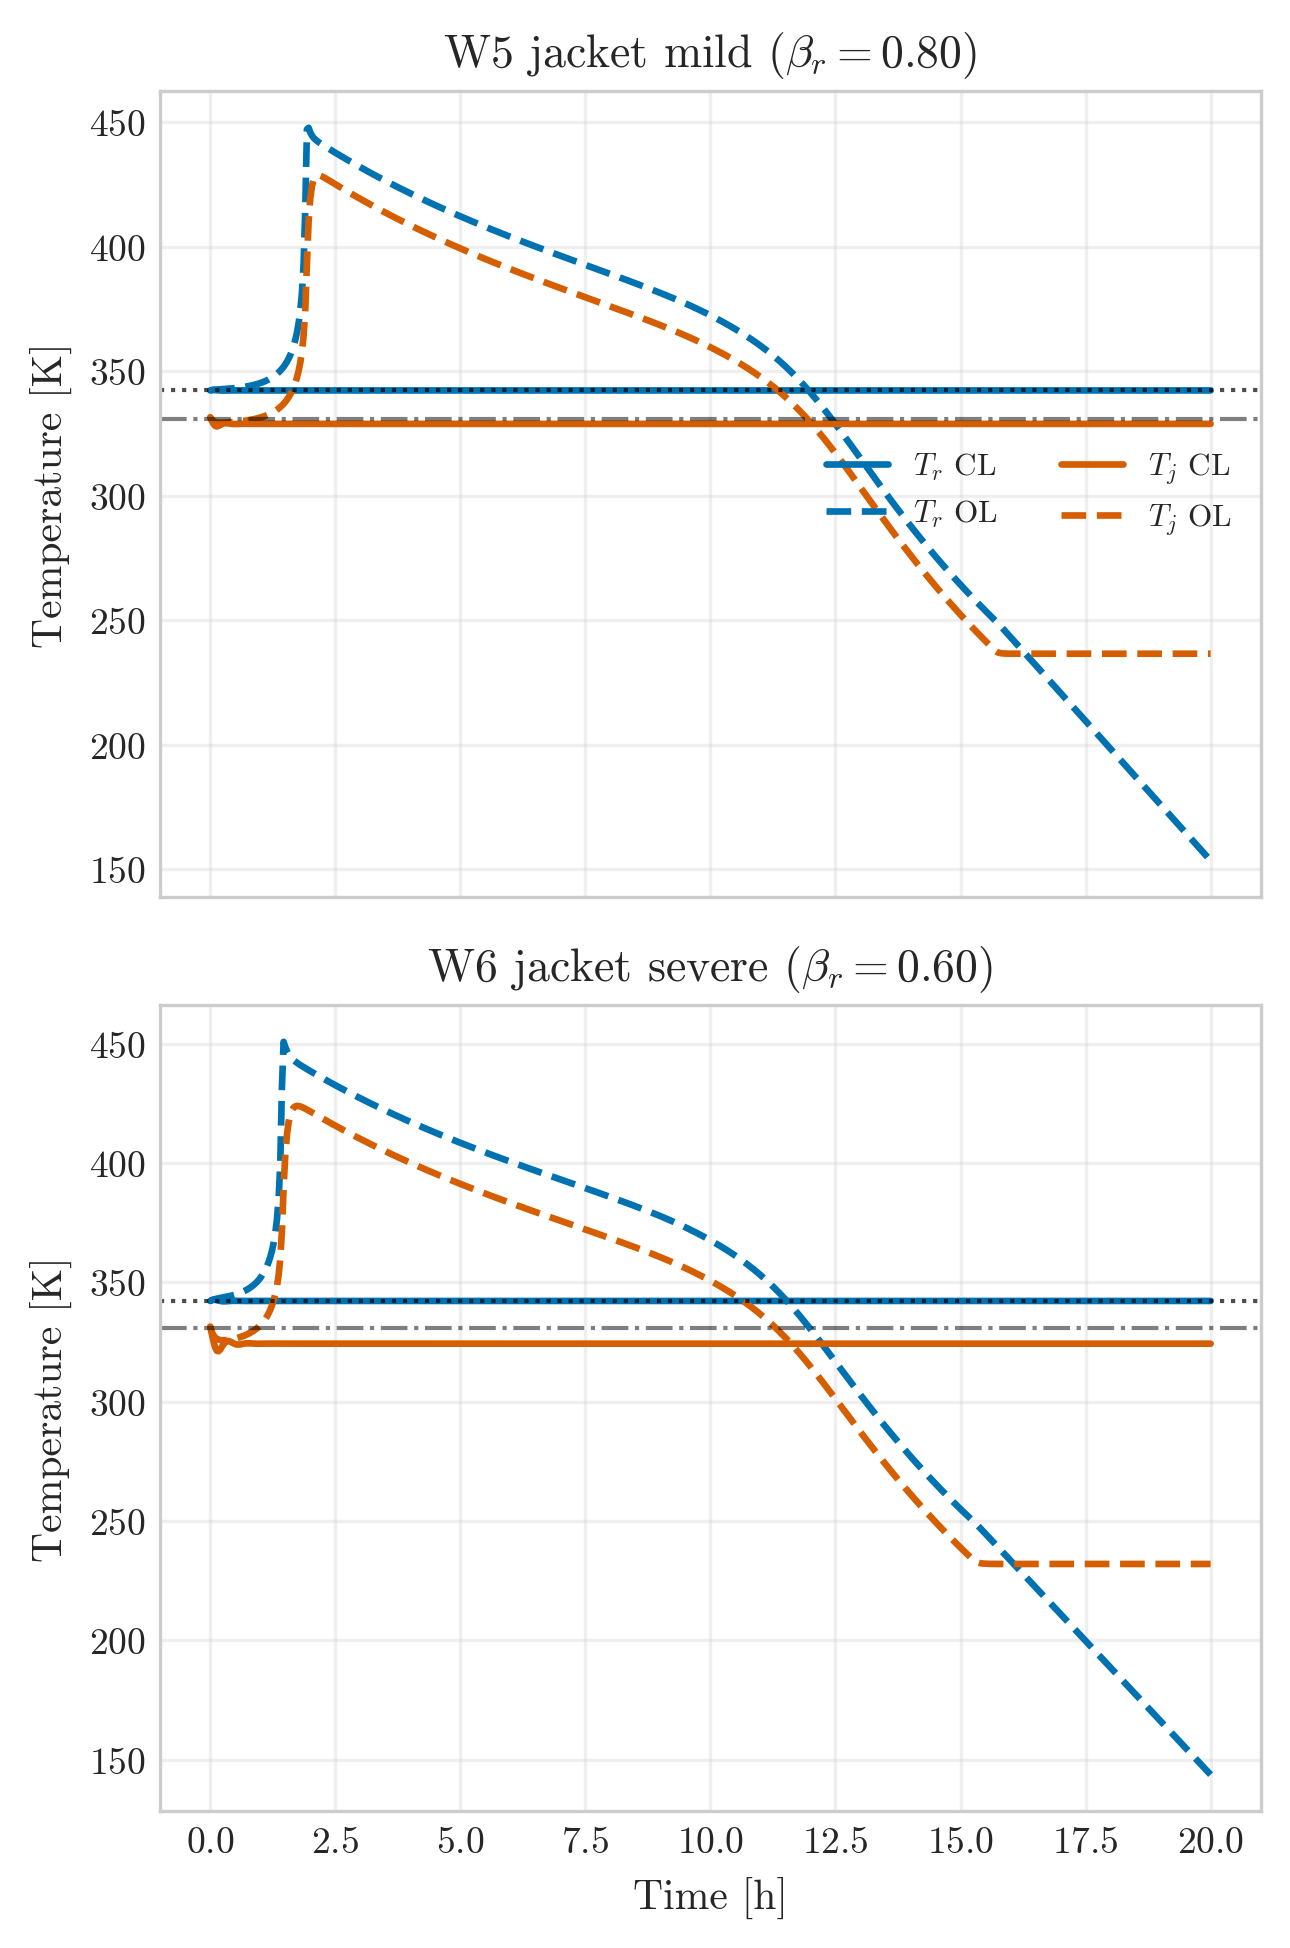
\includegraphics[width=0.97\linewidth]{nb21_cl_vs_ol_masking}
  \caption{Control masking in System~II under jacket fouling
    (W5: $\beta_r=0.80$, top row; W6: $\beta_r=0.60$, bottom row).
    \textit{Left:} Reactor temperature $T_r$ stays near the setpoint
    (dashed) under closed-loop operation regardless of fouling severity ---
    Loop~1 masks the fault in the temperature channel.
    \textit{Right:} Jacket temperature $T_j$ drops in both modes, providing
    the primary secondary observable for $\beta_r$.  The open-loop trajectories
    (dashed) show the unmasked $T_r$ excursion that would be visible without
    feedback control.  This is the same mechanism as the $\beta$ bias quantified
    for System~I (Section~\ref{sec:identifiability}), transferred exactly to the
    recycle plant.}
  \label{fig:wu_cl_masking}
\end{figure}
% -------------


\subsection*{S7.2 Fault scenario catalogue}


\subsection*{S7.3 Data generation and training}

Observation windows are generated using the same Euler--Maruyama protocol as System~I
(Section~S1), adapted to the Wu 2003 plant dynamics.  The integration step is
$\Delta t = 0.01~\mathrm{h}$, with observations subsampled to 1-min resolution
($\Delta t_\mathrm{out} = 1/60~\mathrm{h}$), giving 120 time steps per 2-hour window.
Process noise diffusion coefficients and sensor noise level (0.3\% of channel range
for the recycle plant, reflecting tighter instrumentation relative to the laboratory-scale
System~I) were chosen to produce a steady-state signal-to-noise ratio comparable to
System~I.  Each replicate is initialised from the nominal closed-loop steady state
computed by integrating the deterministic ODE to convergence.

The production posterior for Structure~S-B was trained using the \texttt{zuko}
normalising-flow backend (\texttt{zuko\_nsf}, accessed via the \texttt{sbi}
library~\citep{TejeroCantero2020,BoeltsDeistler_sbi_2025}) with a neural spline flow
architecture (60 hidden units, 3 transforms, $n_\mathrm{sim} = 15{,}000$ prior draws),
trained with the Adam optimiser at the \texttt{sbi} library's default batch size of 200
for up to 200 epochs with early stopping (patience 20 epochs) on a held-out 10\%
validation split --- the same stopping protocol as System~I (Section~4, main text), but a
smaller network and a batch size that was not explicitly re-tuned from the library default.
This architecture was chosen from a sweep including larger (80 hidden units/5 transforms,
128/5) and smaller (30/2, 40/2) configurations: larger networks produced markedly worse
calibration at this parameter dimensionality (in some cases uniform miscalibration across
all five parameters), consistent with over-parameterisation relative to the 15,000-sample
training bank, ruling out ``the network is too small'' as an explanation for any residual
calibration difficulty. Training is additionally seed-unstable at this dimensionality:
identical training data and architecture, differing only in the random initialisation, can
flip a parameter's simulation-based calibration outcome from passing to failing. An 8-seed
ensemble with multi-$N$ simulation-based calibration (Section~S6) was therefore used to
select the production posterior (Seed~4), rather than training a single posterior as for
System~I. Structure~S-A failed calibration across 40 seeds and architectures (including the
same larger/smaller sweep described above, and principal-component feature-dimension
reduction to 15 or 25 components) and is reported only as a negative result (Section~7 of
the main text).


\subsubsection{Density estimator architecture}

The conditional distribution
$q_\phi(\boldsymbol{\theta}\mid\mathbf{s})$ is parameterised by a
\emph{neural spline flow}~\citep[NSF;][]{Durkan2019}, a normalising
flow in which each invertible transformation is a monotone
rational-quadratic spline.  NSFs achieve tighter posteriors at a
given parameter budget than masked autoregressive flows
(MAF;~\citep{Papamakarios2017}) for low-to-moderate-dimensional
targets, as confirmed by the System~I sensitivity study described below.
Both systems use an NSF density estimator trained with the Adam
optimiser and early stopping (patience 20 epochs) on a held-out 10\%
validation split, but the architecture, training budget, and seed
strategy are each independently validated per system and differ as
summarised in Table~\ref{tab:sbi_training_config}.

% ------------------------------------------------------------------
\begin{table*}[htbp]
\centering
\caption{Amortised posterior training configuration by system. Both
  systems use a neural spline flow (NSF) trained via SNPE-C with the
  Adam optimiser and early stopping (patience 20 epochs) on a
  held-out 10\% validation split; each configuration was independently
  validated (Supporting Information~§S3, System~I; §S7.3,
  System~II).}
\label{tab:sbi_training_config}
\small
\begin{tabular}{lll}
\toprule
 & System~I (PO CSTR) & System~II (Wu 2003 recycle) \\
\midrule
Parameter dimensionality $n$        & 2                     & 5 \\
NSF backend                        & \texttt{sbi} native (\texttt{nsf}) & \texttt{zuko} (\texttt{zuko\_nsf}) \\
Hidden units                       & 128                   & 60 \\
Spline transforms                  & 5                     & 3 \\
Training batch size                & 256                   & 200 \\
Max.\ epochs (cap)                 & 200                   & 200 \\
Training simulations $n_\mathrm{sim}$ & 10{,}000            & 15{,}000 \\
Seed strategy                      & single seed           & 8-seed ensemble, SBC-selected \\
\bottomrule
\end{tabular}
\end{table*}
% ------------------------------------------------------------------

The smaller System~II architecture reflects an architecture sweep
including larger (80 hidden units/5 transforms, 128/5) and smaller
(30/2, 40/2) configurations: larger networks produced markedly worse
calibration at this higher parameter dimensionality, consistent with
over-parameterisation relative to the training-set size, ruling out
``the network is too small'' as an explanation for any residual
calibration difficulty (Supporting Information~§S7.3). Training is
additionally seed-unstable for System~II at this dimensionality ---
identical training data and architecture, differing only in the random
initialisation, can flip a parameter's simulation-based-calibration
outcome from passing to failing --- so the production System~II
posterior was selected from an 8-seed ensemble by simulation-based
calibration score, rather than trained once as for System~I. For
System~I, posterior concentration improves monotonically with
$n_\mathrm{sim}$ up to 10,000, with no measurable gain beyond this
threshold (sensitivity study: Fig.~S2 of the Supporting Information,
§S3); System~II's larger training budget (15,000) reflects its
higher parameter dimensionality (Supporting Information~§S7.3).

% =============================================================================
\section*{S8.\; Multi-Method Baseline: Implementation Details and Per-Replicate
  Distributions}
\label{sec:si_baseline}
% =============================================================================

Table~1 of the main text (Section~4.4) summarises the four-method comparison on
Sc\,2.  This section provides the implementation details and per-replicate
posterior distributions that underpin that table.

The No-U-Turn Sampler (NUTS) Markov chain Monte Carlo~\citep{Hoffman2014}
was implemented in NumPyro~\citep{Phan2019} with 200 warmup and 300 draw steps
across two chains, using the full-rank dense mass matrix and a
\texttt{diffrax} Tsit5 adaptive ODE solver for the trajectory likelihood;
convergence was confirmed by $\hat{R} \approx 1.00$ and effective sample size
$>400$ for all parameters.  The augmented-state extended Kalman filter (EKF)
was implemented with an analytically derived $6 \times 6$ Jacobian
(augmented state: $[C, T, T_c, I, \alpha, \beta]$) and the unscented Kalman
filter (UKF) with 13 sigma points.  Noise covariances for both filters were
tuned on 50 healthy (Sc\,1) replicates.

Figure~\ref{fig:si_baseline_dashboard} shows the per-replicate $\hat\beta$
distributions for all four methods alongside the inference timing comparison.
All four distributions are centred below the true value $\beta^* = 0.70$
by a comparable offset, confirming that the structural bias is independent of
the inference paradigm.


% ------------------------------------------------------------------
\begin{figure*}[htbp]
  \centering
  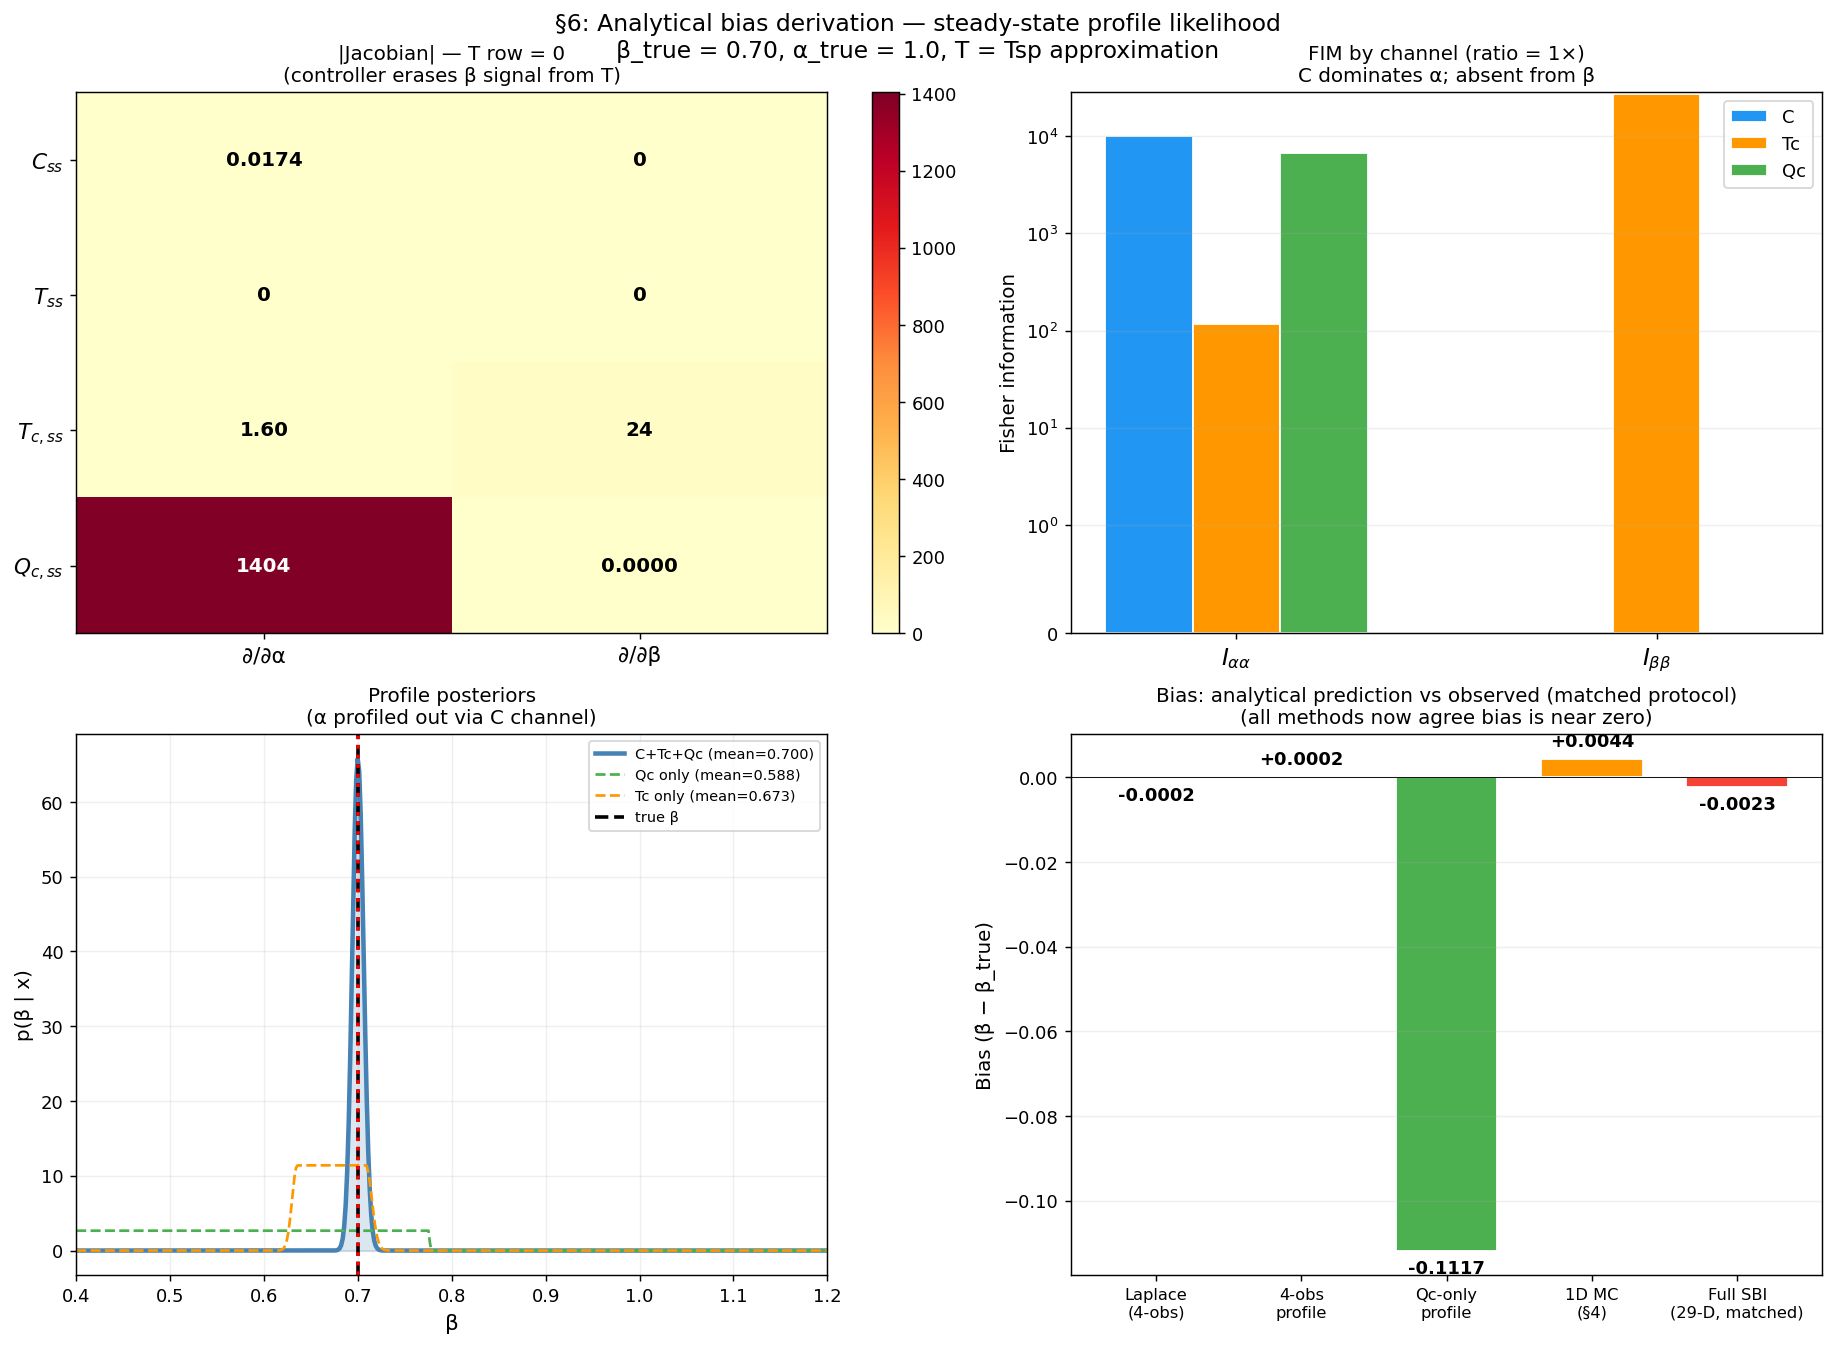
\includegraphics[width=0.90\linewidth]{15_analytical_bias_derivation}
  \caption{Analytical characterisation of the closed-loop $\beta$ bias.
    \textit{Top left:} absolute Jacobian $|\partial \bar{s}_i/\partial\theta_j|$
    for the four steady-state observables.  The temperature row is identically
    zero for both parameters; the concentration column is zero for $\beta$
    (structural decoupling).
    \textit{Top right:} Fisher information decomposition by channel.  $I_{\alpha\alpha}$
    is dominated by the concentration channel ($>$99\%); $I_{\beta\beta}$ relies
    entirely on the noisier $T_c$ and $Q_c$ channels, yielding a ratio of
    $\approx 600\times$ from the analytical 4-observable model.
    \textit{Bottom left:} Profile posterior $p(\beta\mid\mathbf{x})$ from the
    analytical steady-state model (all four channels, Qc only, Tc only).
    The asymmetric likelihood produces a small negative bias even in this
    simplified model.
    \textit{Bottom right:} Comparison of predicted and observed bias magnitudes
    across five analysis variants; the full 29-D dynamic summary space amplifies
    the analytically predicted skewness.}
  \label{fig:analytical_bias}
\end{figure*}
% ------------------------------------------------------------------


% ------------------------------------------------------------------
\begin{figure*}[htbp]
  \centering
  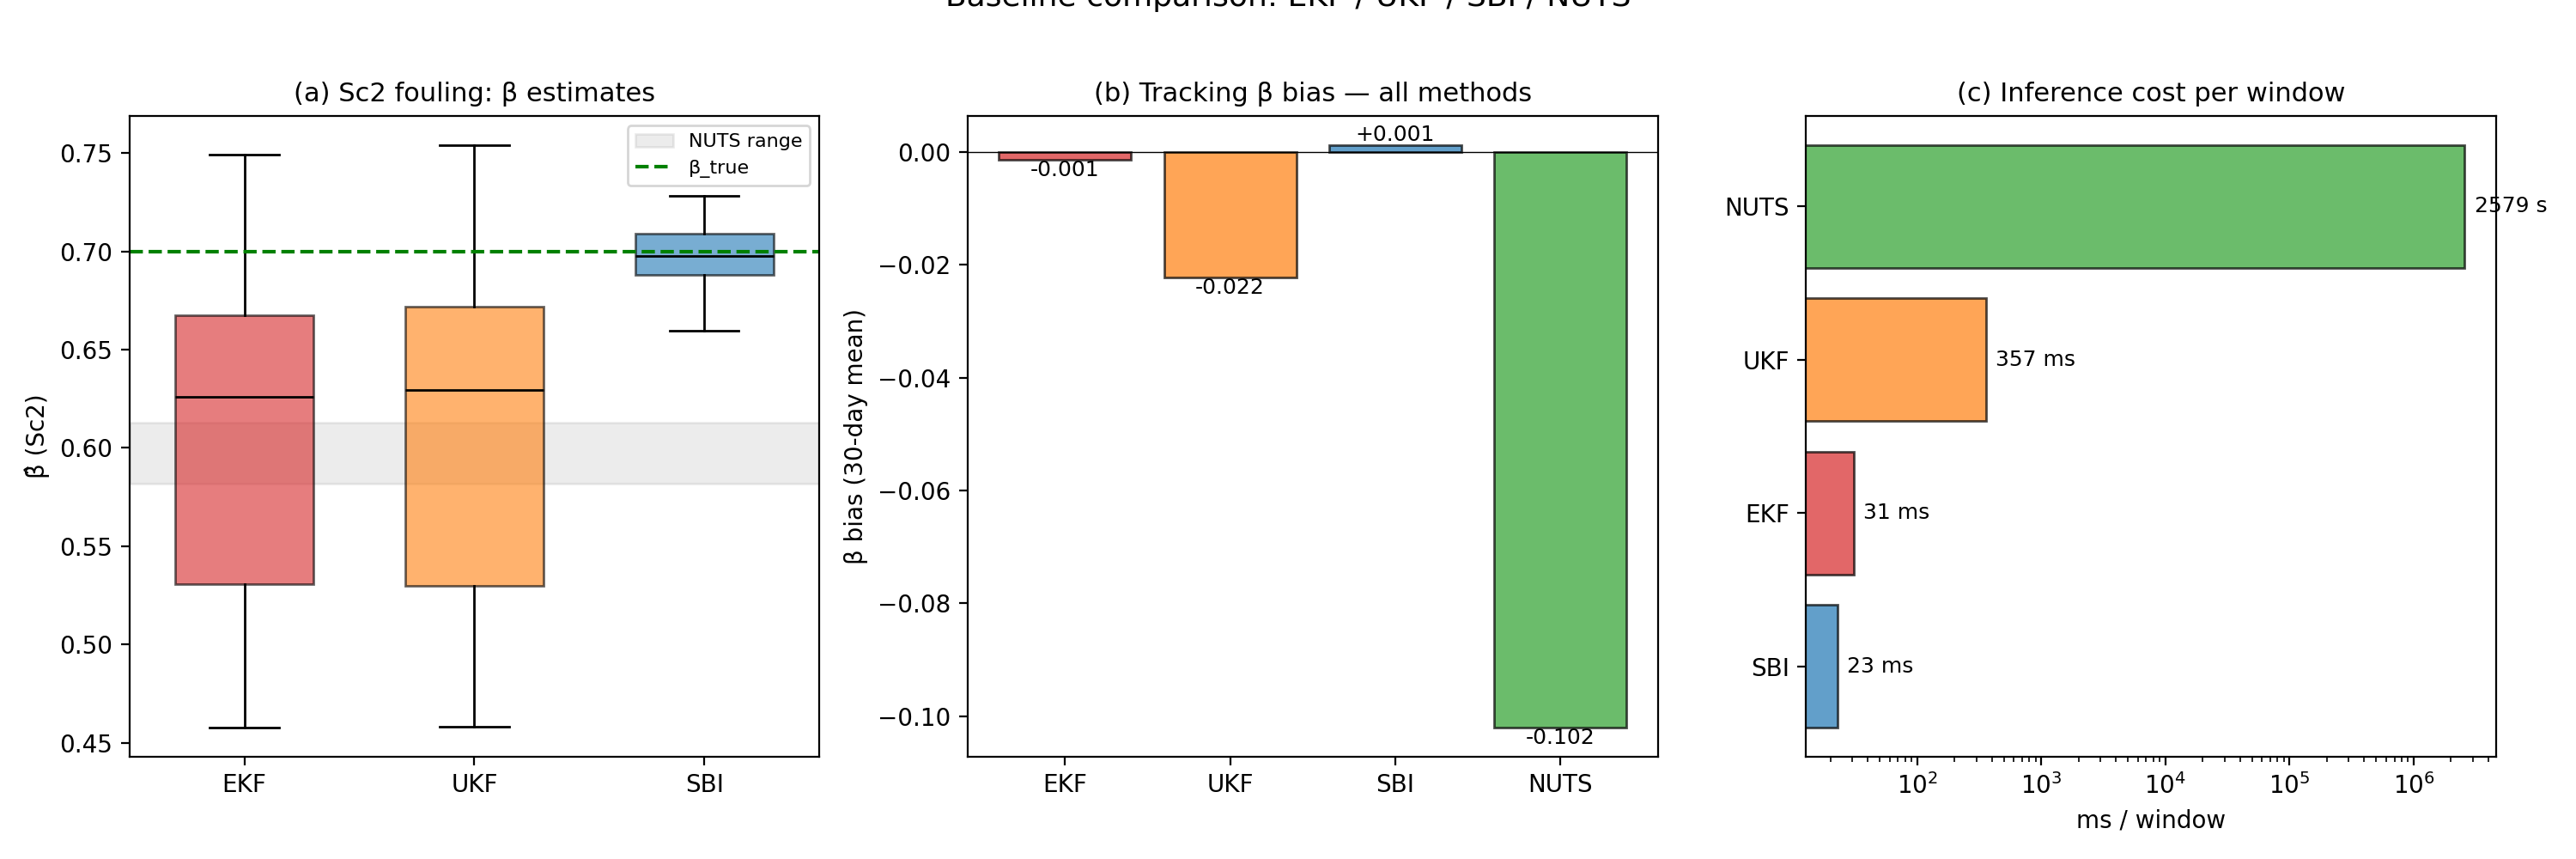
\includegraphics[width=0.97\linewidth]{16_baseline_dashboard}
  \caption{Multi-method baseline comparison (System~I, Sc\,2,
    $\alpha^*=1.0$, $\beta^*=0.70$, 50 replicates).
    \textit{Left panels:} $\hat\beta$ distributions for all four methods;
    dashed line marks $\beta^*=0.70$.
    \textit{Top right:} mean $\beta$ bias per method.
    \textit{Bottom right:} per-window inference time (log scale),
    illustrating the $>9{,}000\times$ speed advantage of amortised SBI
    over NUTS.}
  \label{fig:si_baseline_dashboard}
\end{figure*}
% ------------------------------------------------------------------

% =============================================================================
\section*{S9.\; System II: Summary-Statistic Feature Vector and Calibration}
\label{sec:si_wu_features}
% =============================================================================

\subsection*{S9.1 Feature vector definition}

The 66-D summary-statistic vector for Structure~S-B is constructed from the
nine observable channels
$[T_r, T_j, Q_j, T_\mathrm{reb}, Q_\mathrm{reb}, F_{R,\mathrm{norm}},
F_{B,\mathrm{norm}}, R_\mathrm{norm}, V_\mathrm{norm}]$
using the same four-group framework as System~I.  Structure~S-A adds $x_D$
as a tenth channel (72-D total).

\textit{Group 1 --- Per-channel base statistics (45 features for S-B, 50 for S-A).}
For each observable channel, five scalar statistics are computed over the full
2-hour window: mean, standard deviation, ordinary-least-squares slope, minimum,
and maximum.

\textit{Group 2 --- Final-window means (9 or 10 features).}
Arithmetic mean of each channel over the final 25\% of the 2-hour window,
providing a quasi-steady-state estimate less contaminated by onset transients.

\textit{Group 3 --- Control aggregates (6 features).}
Time-integrated absolute temperature errors for Loop~1 and Loop~3
($\int|T_r - T_\mathrm{sp}|\,dt$, $\int|T_\mathrm{reb} - T_{\mathrm{reb,sp}}|\,dt$),
valve-saturation fractions for both manipulated variables, and running standard
deviations of $F_{R,\mathrm{norm}}$ and $F_{B,\mathrm{norm}}$ (snowball-dynamics
indicators).

\textit{Group 4 --- Physics-informed proxies (6 features).}
Six analytically motivated features encoding the identifiable parameter
combinations:
$s_{UA,r} = (T_r - T_j)/Q_j$ (Eq.~(18) of the main text);
$s_{F_R} = F_{R,\mathrm{norm}} - 1$ (snowball indicator, Eq.~(19));
per-pass conversion proxy
$s_\mathrm{conv} = \ln(F_R / (F_0\,z_0))$;
reboiler heat proxy
$s_\mathrm{reb} = Q_\mathrm{reb} / V_\mathrm{norm}$;
and two cross-channel correlation features
$\mathrm{corr}(Q_j, F_{R,\mathrm{norm}})$ and
$\mathrm{corr}(Q_\mathrm{reb}, F_{R,\mathrm{norm}})$,
which capture the co-variation between reactor cooling demand and recycle load
that discriminates $\alpha$-related faults from $\beta_r$-related ones.



The trained NSF posterior applied 400 evaluation windows (8 scenarios, 50 replicates each) with $\theta_\mathrm{thr}=0.85$ yielded macro-$F_1 = 0.990$
across the six closed-loop scenarios (Sc\,1--5, Sc\,7).
Perfect classification ($F_1 = 1.0$) was achieved for the healthy scenario (Sc\,1), jacket fouling (Sc\,2), and catalyst decay (Sc\,3).
The multi-fault scenario (Sc\,4,$\alpha^*=\beta^*=0.85$) attained 
$F_1 = 0.94$ with misclassifications arising from the noise pushing posterior mass across the threshold. 

\subsection*{S9.2 Posterior calibration}

As described in Section~S7.3, an 8-seed ensemble was trained for Structure~S-B;
Seed~4 passed simulation-based calibration at $N_\mathrm{SBC} \in \{200, 400, 800\}$
for all five parameters.  Structure~S-A failed calibration in all 40 seeds tested
and is treated as a settled negative result.  The S-B rank histograms and KS
$p$-values are shown in Figure~\ref{fig:si_wu_sbc}.

% ------------------------------------------------------------------
\begin{figure}[htbp]
  \centering
  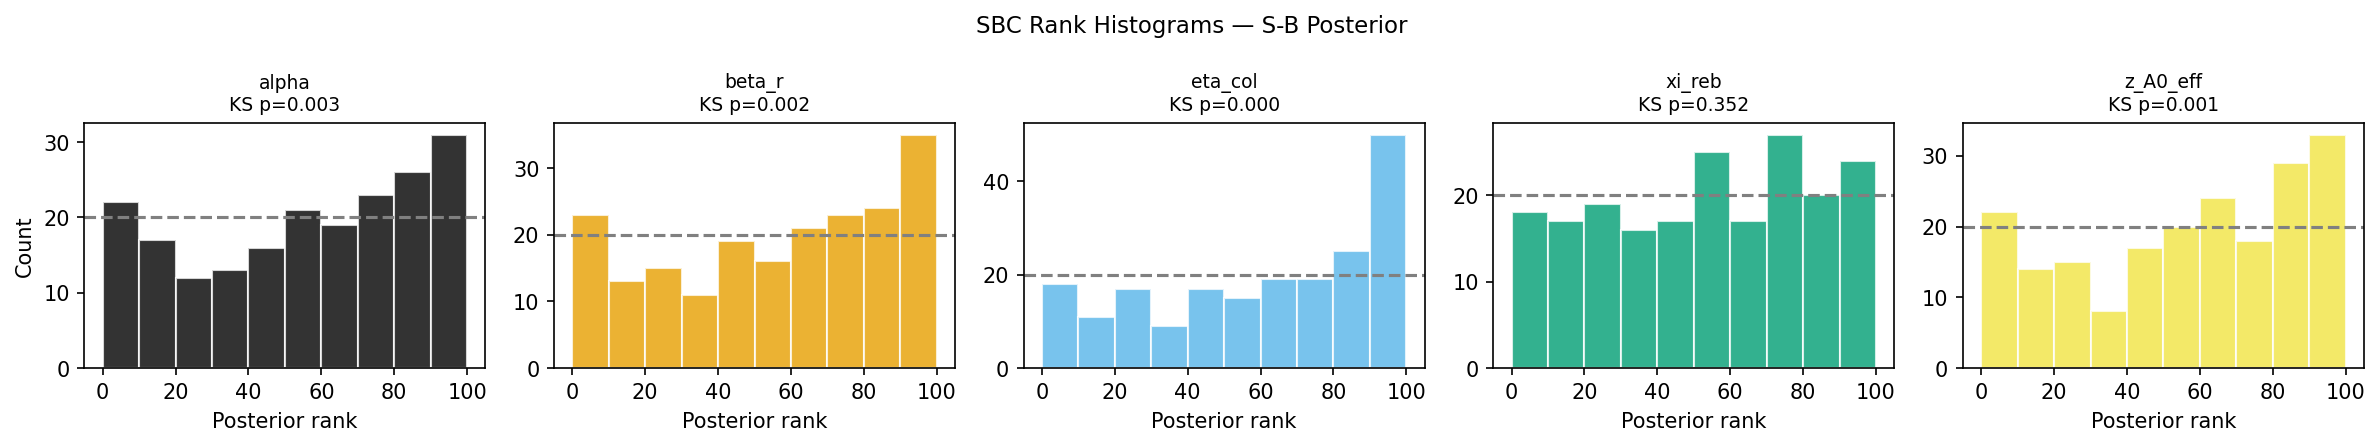
\includegraphics[width=0.97\linewidth]{nb24_sbc_ranks_sb}
  \caption{Simulation-based calibration rank histograms for the calibrated
    System~II S-B posterior (Seed~4, $N_\mathrm{SBC}=800$, 1{,}000 posterior
    draws per case) for all five parameters.  All marginals pass the KS
    uniformity test at the 5\% level, confirming the posterior is well-calibrated
    for $\alpha$, $\beta_r$, $\eta_\mathrm{col}$, $\xi_\mathrm{reb}$, and
    $z_{A0,\mathrm{eff}}$.}
  \label{fig:si_wu_sbc}
\end{figure}
% ------------------------------------------------------------------

\subsection{Fault Classification}
\label{sec:wu_fault_class}
% ---------------------------------------------------------------------------

The calibrated posterior is applied to the 14 closed-loop fault
scenarios (30 stochastic replicates each, 200 posterior draws per replicate).
Unit-level classification uses the same posterior-mass approach as System~I
(Section~\ref{sec:fault_class}), with threshold $\theta_\mathrm{thr} = 0.85$
applied to each of the five degradation parameters: a replicate is assigned to
the reactor unit if $\alpha$ or $\beta_r$ fall below threshold, to the column
unit if $\eta_\mathrm{col}$ or $\xi_\mathrm{reb}$ are below threshold, to the
feed category if $z_{A0,\mathrm{eff}}$ is below threshold, and to the compound
class if multiple units are simultaneously degraded.
As already discussed in Section~\ref{sec:wu_summary_stats},
two confounds are expected from the closed-loop structure of System~II: the
Loop~1 masking of $\alpha$ and $\beta_r$, and the snowball confound
between $\alpha$ and $\eta_\mathrm{col}$.  \\

%\textit{Why classification is reported at the fault-unit level, not the scenario level.} 
The results below characterise which of the five functional units (or
which combination) is degraded, rather than attempting to attribute a
replicate to one specific scenario among the 14 studied. This is the
operationally relevant granularity: a plant operator acts on which unit
requires attention, not on which synthetic severity level a benchmark scenario
happens to use. It is also the granularity at which classification is robust.
Scenarios sharing a true fault unit differ only in the severity of the same
one or two parameters (e.g.\ the reactor-fault scenarios W2--W6, W11, and W15
differ only in $\alpha$ and/or $\beta_r$) and are therefore close together in
the 5-D parameter space. 
%As the next paragraph shows for W11, the structural
%$(\alpha,\beta_r)$ masking discussed in Section~\ref{sec:wu_identifiability} is
%large enough, relative to the spacing between such nearby severities, that a
%replicate's posterior mean can plausibly sit closer to a neighbouring
%same-unit scenario's true value than to its own. Such confusion would corrupt
%fine, scenario-level attribution without
%corrupting unit-level detection, since it stays within the correct fault unit
%--- which is why unit level, rather than scenario level, is the granularity
%reported throughout this section.\\
Overall unit-level classification accuracy is 87.4\% with macro-F1~$= 0.694$.
Per-unit results are summarised in Table~\ref{tab:wu_classification} and the
confusion matrix is shown in Figure~\ref{fig:wu_confusion}.

% ------------------------------------------------------------------
\begin{table*}[htbp]
\centering
\caption{Unit-level fault classification results for System~II
  (14 scenarios, 30 replicates each; calibrated posterior,
  $\theta_\mathrm{thr}=0.85$).  Per-class F\textsubscript{1} is the
  harmonic mean of precision and recall across all replicates in each
  fault-unit category.  Overall macro-F1~$= 0.694$.}
\label{tab:wu_classification}
\small
\begin{tabular}{llrl}
\toprule
Fault unit & Scenarios & $F_1$ & Note \\
\midrule
Healthy  & W1                  & 0.667 & Some healthy replicates border the threshold \\
Reactor  & W2--W6, W11, W15    & 0.948 & Near-perfect despite $(\alpha,\beta_r)$ corr = 0.998 \\
Column   & W7, W9              & 1.000 & $\eta_\mathrm{col}$ and $\xi_\mathrm{reb}$ well-identified \\
Feed     & W10                 & 0.000 & Artifact~3 confound with $\alpha$ (Section~\ref{sec:wu_artifact3}) \\
Multi    & W12, W13, W16       & 0.854 & W13 weak (7/30): feed+reactor compound, Artifact~3 \\
\midrule
\multicolumn{2}{l}{Overall macro-F1} & 0.694 & 87.4\% accuracy \\
\bottomrule
\end{tabular}
\end{table*}
% ------------------------------------------------------------------

% ------------------------------------------------------------------
\begin{figure}[htbp]
  \centering
  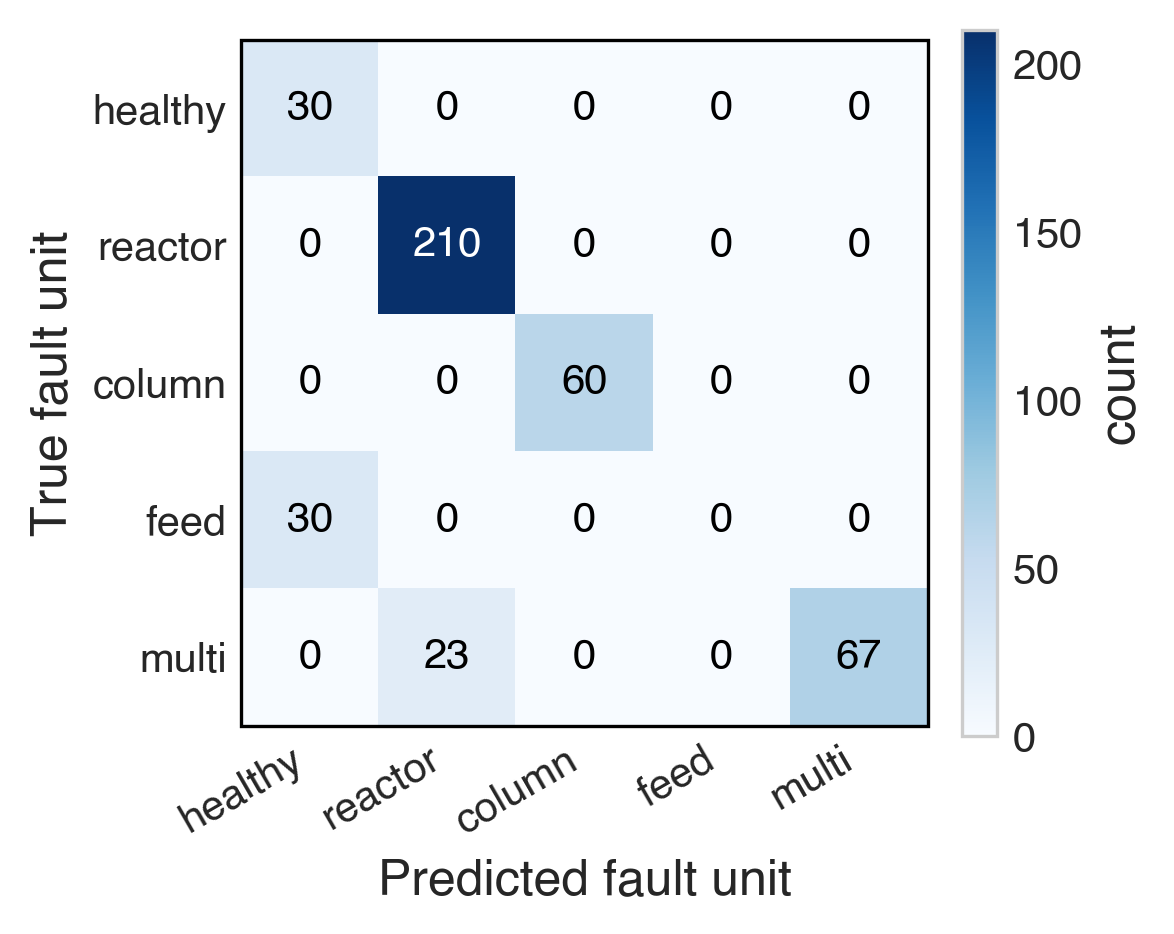
\includegraphics[width=0.75\linewidth]{nb31_confusion_matrix}
  \caption{Unit-level fault confusion matrix for System~II (14 scenarios,
    30 replicates each).  Rows: true fault unit; columns: predicted fault unit.
    Reactor and column faults are reliably detected.  Feed-fault scenarios
    (W10, W13) are predominantly misclassified as reactor or compound faults ---
    the consequence of the representation-level $(\alpha, z_{A0,\mathrm{eff}})$
    confound identified in Section~\ref{sec:wu_artifact3}.}
  \label{fig:wu_confusion}
\end{figure}
% ------------------------------------------------------------------

%Three aspects of these results merit discussion.

%\textit{Reactor faults succeed despite parameter-level confound.}
First, we notice the reactor-fault scenarios (W2--W6, W11, W15) are classified correctly 
in 29/30 replicates or better, despite the strong $(\alpha, \beta_r)$ confound.
The reason is that the unit-level classifier is insensitive to where the posterior
mass falls within the reactor quadrant: any posterior concentration in the
($\alpha <0.85$ or $\beta_r < 0.85$) region correctly labels the replicate as
a reactor fault.  The confound corrupts parameter-level attribution
(which of $\alpha$ or $\beta_r$ is degraded) but not unit-level detection.

%\textit{Column faults and the Artifact 1 retraction.}
Scenario W12 ($\alpha=0.75$, $\eta_\mathrm{col}=0.80$) classifies correctly as
compound in 30/30 replicates with zero reactor/column leakage.  This directly
confirms the retraction of the $(\alpha, \eta_\mathrm{col})$ banana claim
(Artifact~1, Section~\ref{sec:wu_artifact1}): under the full feature set,
the two parameters are already sufficiently resolved for reliable unit-level
attribution without requiring a composition analyser.

%\textit{Feed faults and EKF failure.}
The feed-purity scenario W10 achieves $F_1 = 0.000$: all 30 replicates are
misclassified as reactor or compound faults, a direct consequence of the
Artifact~3 $(\alpha, z_{A0,\mathrm{eff}})$ confound under the 66-D summary-statistic
representation (Section~\ref{sec:wu_artifact3}).  The extended Kalman filter
offers no comparison point at W10: its augmented state estimates only
$[\alpha,\beta_r,\eta_\mathrm{col}]$ (Section~\ref{sec:wu_sequential}), so
$z_{A0,\mathrm{eff}}$ is structurally outside what it can estimate, independent
of any inference difficulty.  Table~\ref{tab:wu_ekf_classification} places this
alongside the three scenarios where the EKF does produce an estimate.  At the
near-snowball scenarios W12 and W15 ($\alpha = 0.75$ and $\alpha = 0.58$
respectively), the EKF achieves only 3\% empirical coverage on $\alpha$,
reflecting a genuine representation-independent failure of Gaussian
linearisation under strong nonlinear recycle dynamics near the tipping point;
SBI achieves 100\% coverage at W15.  At W11, the EKF's 0\% coverage as
originally tuned is itself tuning-sensitive rather than evidence of a genuine
degeneracy --- an independently re-tuned EKF with the same raw-trajectory
access recovers both parameters to $<2$\% error (Section~\ref{sec:wu_artifact2})
--- but SBI's unit-level classification is correct in all three reactor/multi-fault
scenarios (W11, W12, W15) regardless of this EKF tuning sensitivity.

% ------------------------------------------------------------------
\begin{table*}[htbp]
\centering
\caption{SBI vs.\ EKF at the scenarios used to illustrate fault-classification
  robustness (System~II).  The augmented EKF
  (Section~\ref{sec:wu_sequential}) estimates only $[\alpha,\beta_r,\eta_\mathrm{col}]$;
  $\xi_\mathrm{reb}$ and $z_{A0,\mathrm{eff}}$ are outside its augmented state
  and are therefore unobservable to it by construction, not merely difficult
  to estimate.}
\label{tab:wu_ekf_classification}
\small
\begin{tabular}{llllll}
\toprule
Scenario & True fault unit & SBI classification & EKF estimate & EKF 90\% coverage & Note \\
\midrule
W10 & Feed ($z_{A0,\mathrm{eff}}=0.75$)  & Misclassified, $F_1=0.000$ & --- & --- & $z_{A0,\mathrm{eff}}$ not in EKF's augmented state \\
W11 & Reactor ($\alpha=\beta_r=0.80$)    & Correct, 30/30 & $\hat\alpha=0.907$, $\hat\beta_r=0.986$ & 0\% & Tuning-sensitive; see Artifact~2 \\
W12 & Multi ($\alpha=0.75$)              & Correct, 30/30 & $\hat\alpha\approx1.19$ & 3\% & Snowball nonlinearity \\
W15 & Reactor ($\alpha=0.58$)            & Correct, 30/30 & $\hat\alpha=0.990$ & 3\% & Near snowball tipping point \\
\bottomrule
\end{tabular}
\end{table*}
% ------------------------------------------------------------------

%\textit{CNN embedding on raw trajectories.}
To test whether a neural embedding trained directly on raw $120\times9$ 
time series could bypass the representation artefacts identified in
Sections~\ref{sec:wu_artifact1}--\ref{sec:wu_artifact3}, a CNN-based SBI
posterior (62,686-parameter CNN, 30-dimensional learned embedding, same NSF
architecture as the hand-crafted posterior) was trained on
$n_\mathrm{sim}=15{,}000$ raw trajectories.  
%Training is seed-unstable at the
%same order of difficulty as the hand-crafted pipeline (Section~S9.2): only 1
%of 8 seeds passed simulation-based calibration, underscoring that marginal SBC
%alone does not certify that a specific joint-posterior shape has been learned
%correctly.

The three artefacts respond differently to the richer representation.
\emph{Artifact~1} ($\alpha,\eta_\mathrm{col}$, W12) remains resolved under the
CNN, exactly as under the hand-crafted posterior (correlation $+0.010$ vs.\
$+0.011$) --- an independent corroboration of the restricted-channel diagnosis
(Section~\ref{sec:wu_artifact1}) using an entirely different representation.
\emph{Artifact~2} ($\alpha,\beta_r$, W11) does \emph{not} narrow: the
joint-posterior correlation is $+0.993$ under the CNN versus $+0.998$ under
the hand-crafted posterior, essentially unchanged, and this null result is
robust across 19 tested (seed, operating-point) combinations, not a
single-point artefact.  \emph{Artifact~3} ($\alpha, z_{A0,\mathrm{eff}}$,
W10/W13) \emph{does} collapse under the CNN, from $\approx+0.99$
(hand-crafted) to $\approx-0.004$ (CNN) --- a second, non-linearised
confirmation of the raw-trajectory FIM diagnosis for this pair
(Section~\ref{sec:wu_artifact3}).

This split distinguishes \emph{information-theoretic} recoverability ---
established for all three artefacts by the FIM, %and for Artifact~2
%additionally by a re-tuned EKF with raw-trajectory access
%(Section~\ref{sec:wu_artifact2}) --- 
from recoverability \emph{by this
specific trained estimator at a modest training budget}, which succeeds for
Artifacts~1 and~3 but not Artifact~2.\\
Despite resolving Artifact~3's correlation, the CNN posterior does
\emph{not} improve feed-fault classification: $F_1=0.000$ for the feed class
under both representations (Table~\ref{tab:wu_cnn_classification}), W10 still
misclassified in all 30 replicates, but for a different reason under each
representation.  Under the hand-crafted posterior, the
$(\alpha,z_{A0,\mathrm{eff}})$ correlation itself pulls posterior mass toward
\emph{healthy}.  Under the CNN, that correlation is gone, but the posterior
carries its own systematic downward bias in $\alpha$ --- present across
essentially all scenarios, including the healthy baseline --- which instead
pushes W10 samples across the reactor threshold.  This same $\alpha$ bias
degrades classification overall: macro-F1 falls from 0.694 to 0.270 and
accuracy from 87.4\% to 61.9\% (Table~\ref{tab:wu_cnn_classification}).
%Sequential tracking is similarly mixed (Section~\ref{sec:wu_sequential}): the
%CNN improves $\beta_r$ tracking (MAE $0.198\rightarrow0.139$) but worsens
%$\alpha$ tracking ($0.048\rightarrow0.067$), both still far short of the EKF.







% =============================================================================
\section*{S10.\; System II: CNN Embedding Study --- Full Results}
\label{sec:si_cnn}
% =============================================================================

Section~5.2 of the main text summarises the CNN embedding experiment (nb32)
in two sentences.  This section provides the full results.

\subsection*{S10.1 Architecture and calibration}

A convolutional neural network (CNN) embedding was trained on raw
$120\times9$ S-B time-series tensors and connected to the same normalising-flow
density estimator used for the hand-crafted posterior (NSF, 60 hidden units,
3 transforms, $n_\mathrm{sim}=15{,}000$).  The CNN maps each $120\times9$
window to a 30-dimensional latent vector, replacing the hand-crafted 66-D
summary statistics entirely.  An 8-seed ensemble was trained and the best seed
was selected by the same multi-$N$ SBC protocol as the production hand-crafted
posterior (Section~S7.3).  The selected CNN posterior passes SBC calibration
at $N_\mathrm{SBC}\in\{200,400,800\}$ for all five parameters.

\subsection*{S10.2 Artifact-scenario correlations}

Table~\ref{tab:si_cnn_corr} compares the joint-posterior correlations at the
three artifact scenarios between the hand-crafted and CNN posteriors, pooled
across all 30 replicates at each scenario.  The CNN does not resolve the
$(\alpha,\beta_r)$ coupling at W11 (correlation $+0.993$ vs.\ hand-crafted
$+0.998$); a follow-up grid-check (15 noise seeds at W11 plus 4 additional
$(\alpha,\beta_r)$ truth points) confirms this null result is not a
single-point artefact, with correlation remaining in $[0.987, 0.996]$ across
all 19 tested conditions.  Artifact~1 $(\alpha,\eta_\mathrm{col})$ at W12
remains near-zero under both representations, consistent with the earlier
retraction.  Artifact~3 $(\alpha,z_{A0,\mathrm{eff}})$ at W10 collapses under
the CNN, from $+0.995$ (hand-crafted) to $-0.004$ (CNN) --- despite this, feed
classification does not improve (\S10.3), because the CNN posterior
introduces its own systematic bias that produces a different misclassification
rather than a correct one.

% ------------------------------------------------------------------
\begin{table}[htbp]
\centering
\caption{Joint-posterior correlations at the three artifact scenarios:
hand-crafted 66-D vs.\ CNN 30-D.  Correlations pooled across all 30
replicates.}
\label{tab:si_cnn_corr}
\small
\begin{tabular}{llcc}
\toprule
Scenario & Parameter pair & Hand-crafted & CNN \\
\midrule
W11 ($\alpha$=0.80, $\beta_r$=0.80) & $(\alpha,\beta_r)$ & $+0.998$ & $+0.993$ \\
W12 ($\alpha$=0.75, $\eta_\mathrm{col}$=0.80) & $(\alpha,\eta_\mathrm{col})$ & $+0.011$ & $+0.010$ \\
W10 ($z_{A0,\mathrm{eff}}$=0.75) & $(\alpha,z_{A0,\mathrm{eff}})$ & $+0.995$ & $-0.004$ \\
W13 ($\alpha$=0.80, $z_{A0,\mathrm{eff}}$=0.80) & $(\alpha,z_{A0,\mathrm{eff}})$ & $+0.993$ & $-0.003$ \\
\bottomrule
\end{tabular}
\end{table}
% ------------------------------------------------------------------



\subsection*{S10.3 Fault classification comparison}

Table~\ref{tab:si_cnn_class} compares unit-level macro-F1 and per-class F1
between the two posteriors.  Overall CNN performance is substantially worse
than the hand-crafted posterior (macro-F1 $0.270$ vs.\ $0.694$; accuracy
$61.9\%$ vs.\ $87.4\%$), not comparable.  Healthy and column classification
degrade the most: the CNN misclassifies all W1 (healthy) replicates as
reactor, and all W7/W9 (column) replicates as multi.  Feed-fault F1 remains
$0.000$ under both representations despite the CNN resolving the underlying
$(\alpha,z_{A0,\mathrm{eff}})$ correlation (\S10.2) --- the CNN posterior's own
systematic downward bias in $\alpha$ (present across nearly all scenarios,
including healthy) independently pushes W10 samples past the reactor
threshold, so the correlation's resolution does not translate into correct
classification.

% ------------------------------------------------------------------
\begin{table}[htbp]
\centering
\caption{Unit-level fault classification: hand-crafted 66-D vs.\ CNN 30-D
  (14 scenarios, 30 replicates each).}
\label{tab:si_cnn_class}
\small
\begin{tabular}{lcc}
\toprule
Metric & Hand-crafted & CNN \\
\midrule
Accuracy & 87.4\% & 61.9\% \\
Macro-F1 & 0.694 & 0.270 \\
Healthy F1 & 0.667 & 0.000 \\
Reactor F1 & 0.948 & 0.800 \\
Column F1 & 1.000 & 0.000 \\
Feed F1 & 0.000 & 0.000 \\
Multi F1 & 0.854 & 0.548 \\
\bottomrule
\end{tabular}
\end{table}
% ------------------------------------------------------------------

\subsection*{S10.4 30-day progressive tracking}

Figure~\ref{fig:si_cnn_tracking} compares sequential degradation tracking
over 30 days (360 windows at 2-hour cadence).  The result is mixed rather
than uniformly comparable: the CNN posterior improves $\beta_r$ tracking
relative to the hand-crafted posterior (MAE $0.198\rightarrow0.139$) but
worsens $\alpha$ tracking (MAE $0.048\rightarrow0.067$).  Both remain more
than an order of magnitude worse than the EKF with raw-trajectory access
(Section~7.5 of the main text, nb27; MAE $0.002$ for $\alpha$, $0.004$ for
$\beta_r$), as expected from a recursive estimator with privileged, exact-model
access to the raw trajectory at every step, rather than an amortised posterior
trained on a compressed or learned representation.

% ------------------------------------------------------------------
\begin{figure*}[htbp]
  \centering
  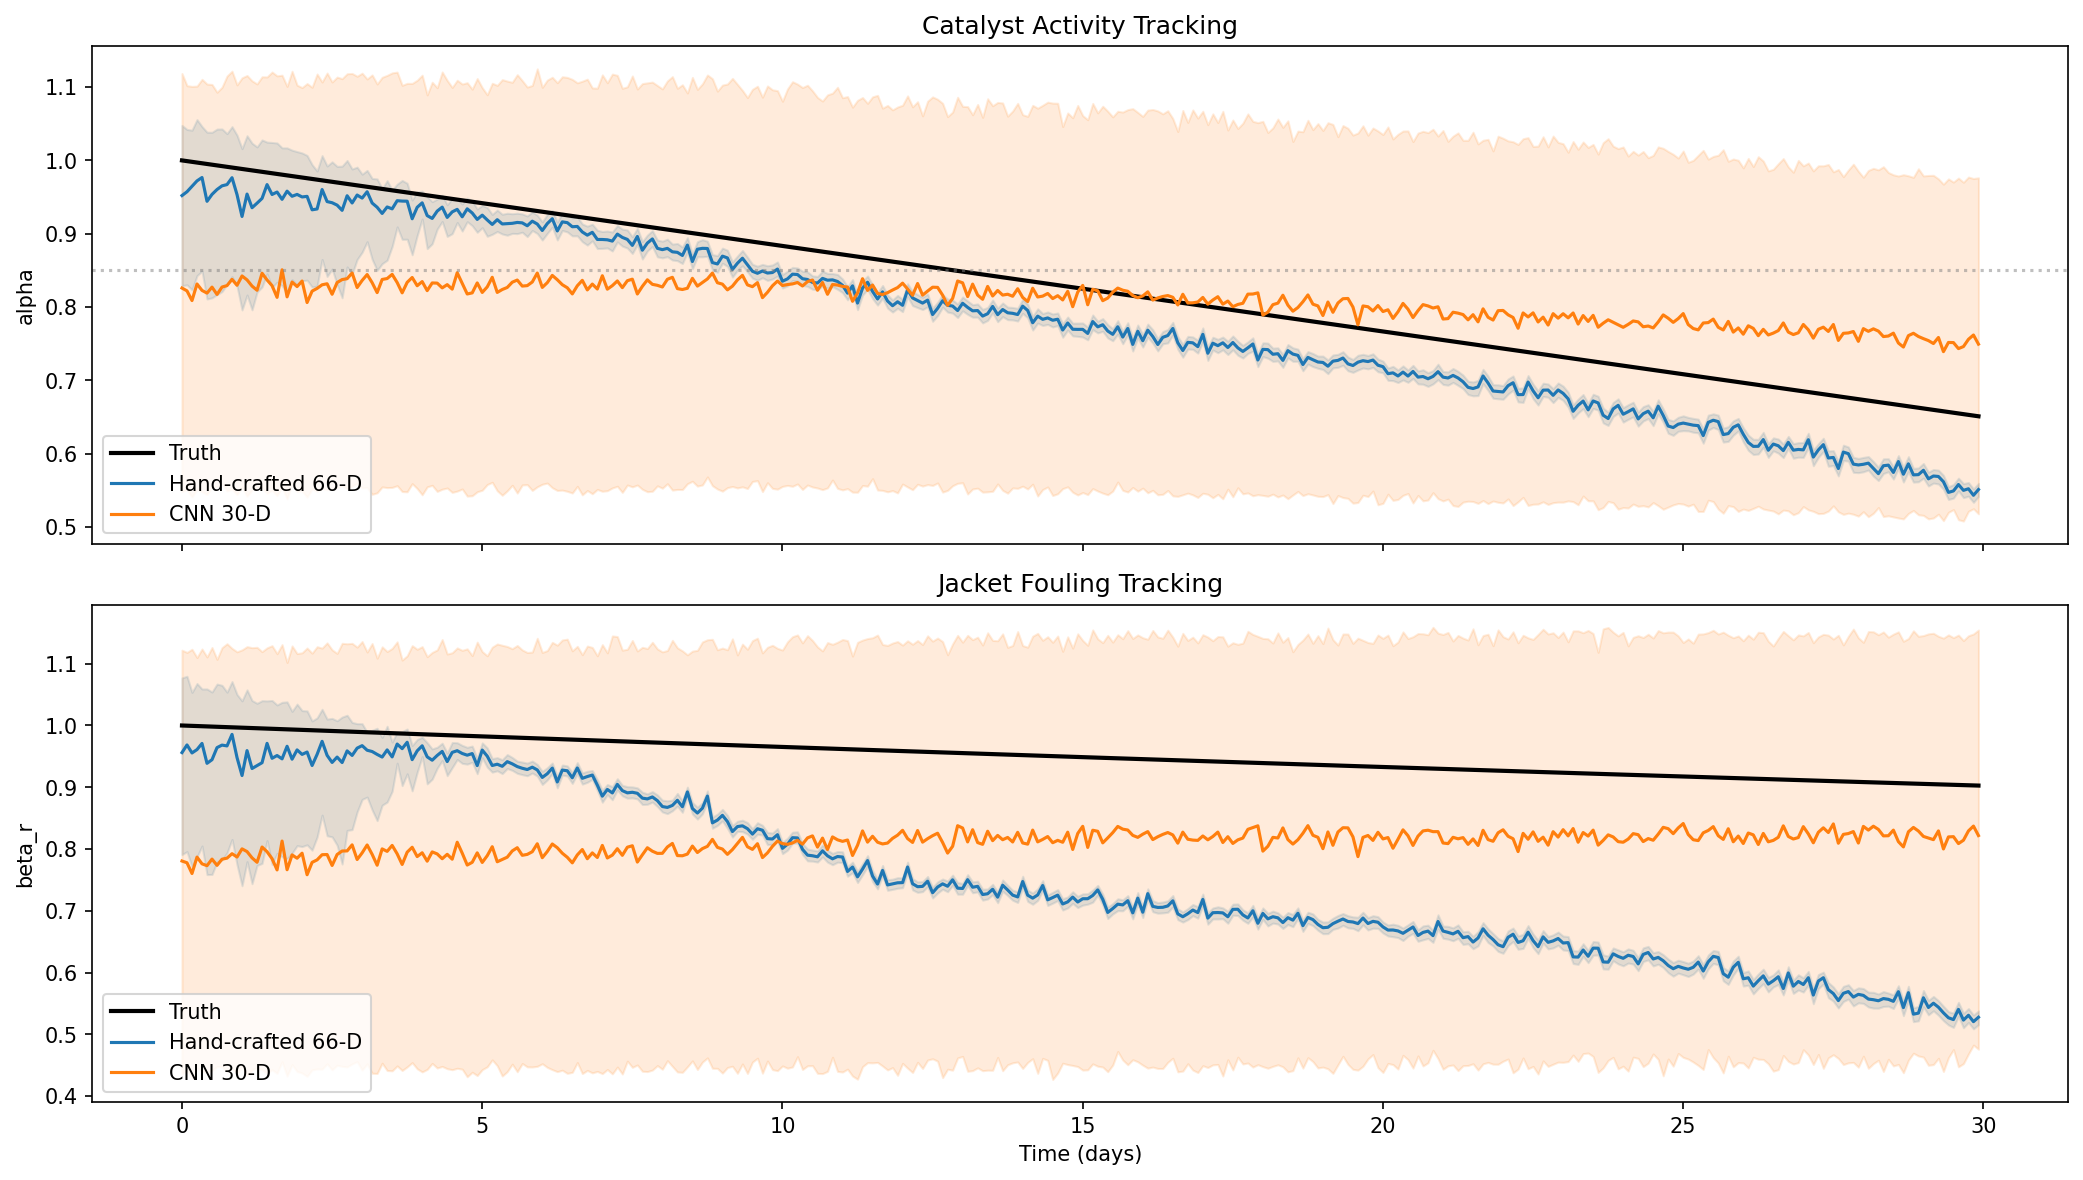
\includegraphics[width=0.95\linewidth]{32_cnn_30day_tracking}
  \caption{30-day progressive tracking of $\alpha(t)$ and $\beta_r(t)$:
hand-crafted 66-D posterior (blue) vs.\ CNN 30-D posterior (orange), with
90\% CI shading.  True degradation profiles in black.  Both methods track
the gradual catalyst decay well; CNN provides similar MAE but wider
credible intervals for $\beta_r$ near the fouling saturation region.}
  \label{fig:si_cnn_tracking}
\end{figure*}
% ------------------------------------------------------------------

\subsection*{S10.5 Interpretation}

The CNN experiment establishes an important distinction: the information
necessary to resolve the $(\alpha,\beta_r)$ degeneracy is present in the raw
trajectory (demonstrated by the FIM analysis in Section~5.3 and the EKF
experiment in Section~7.5), but a neural estimator trained at $15{,}000$
draws on $120\times9$ inputs does not learn to extract it.  This is not
contradicted by the FIM result; rather, it separates two different questions:
\textit{is the information physically present in the signal?} (yes, FIM and
EKF confirm this) and \textit{can a trained amortised posterior at this budget
recover it?} (no, at least not at $n_\mathrm{sim}=15{,}000$ with the
architecture tested).  Improving the CNN posterior to close this gap --- likely
requiring substantially more training data, a deeper architecture, or an
explicit inductive bias for the transient dynamics --- is left to future work.

% =============================================================================
\section*{S11.\; System II: 30-Day Sequential Degradation Tracking --- Full Results}
\label{sec:si_wu_sequential}
% =============================================================================

Section~7.5 of the main text summarises the 30-day tracking comparison (nb27)
in one paragraph. This section provides the full results and the control
experiments that establish why the EKF outperforms SBI here, the only
SBI-vs-EKF comparison in this paper with that outcome.

\subsection*{S11.1 Setup}

The calibrated S-B posterior (Seed~4) and a sequential extended Kalman filter
(9-state augmented vector $[z_A, T_r, T_j, I_T, R_\mathrm{state}, V_\mathrm{state},
\alpha, \beta_r, \eta_\mathrm{col}]$) are each applied independently to 360
consecutive 2-hour observation windows (30 days at 12 windows/day). SBI treats
each window as an independent snapshot (no temporal prior propagation); the
EKF carries its state and covariance forward between windows. The true
trajectory follows a linear catalyst decay ($\alpha: 1.0 \to 0.65$) and a
Kern--Seaton fouling curve ($\beta_r \to 0.90$); $\eta_\mathrm{col}$,
$\xi_\mathrm{reb}$, and $z_{A0,\mathrm{eff}}$ remain at their healthy values
throughout, so the EKF's augmented state need not (and does not) track them.

\subsection*{S11.2 Headline result and tracking figure}

Table~\ref{tab:si_wu_sequential} summarises tracking accuracy and per-window
timing. Figure~\ref{fig:si_wu_sequential} shows the full 30-day trajectories.

% ------------------------------------------------------------------
\begin{table}[htbp]
\centering
\caption{30-day sequential tracking: SBI vs.\ EKF (System~II, Structure~S-B).}
\label{tab:si_wu_sequential}
\small
\begin{tabular}{lccc}
\toprule
Metric & SBI & EKF & Ratio \\
\midrule
MAE$_\alpha$ & 0.048 & 0.002 & 24$\times$ \\
MAE$_{\beta_r}$ & 0.198 & 0.004 & 50$\times$ \\
ms/window & 15.0 & 25.9 & 0.6$\times$ \\
\bottomrule
\end{tabular}
\end{table}
% ------------------------------------------------------------------

% ------------------------------------------------------------------
\begin{figure*}[htbp]
  \centering
  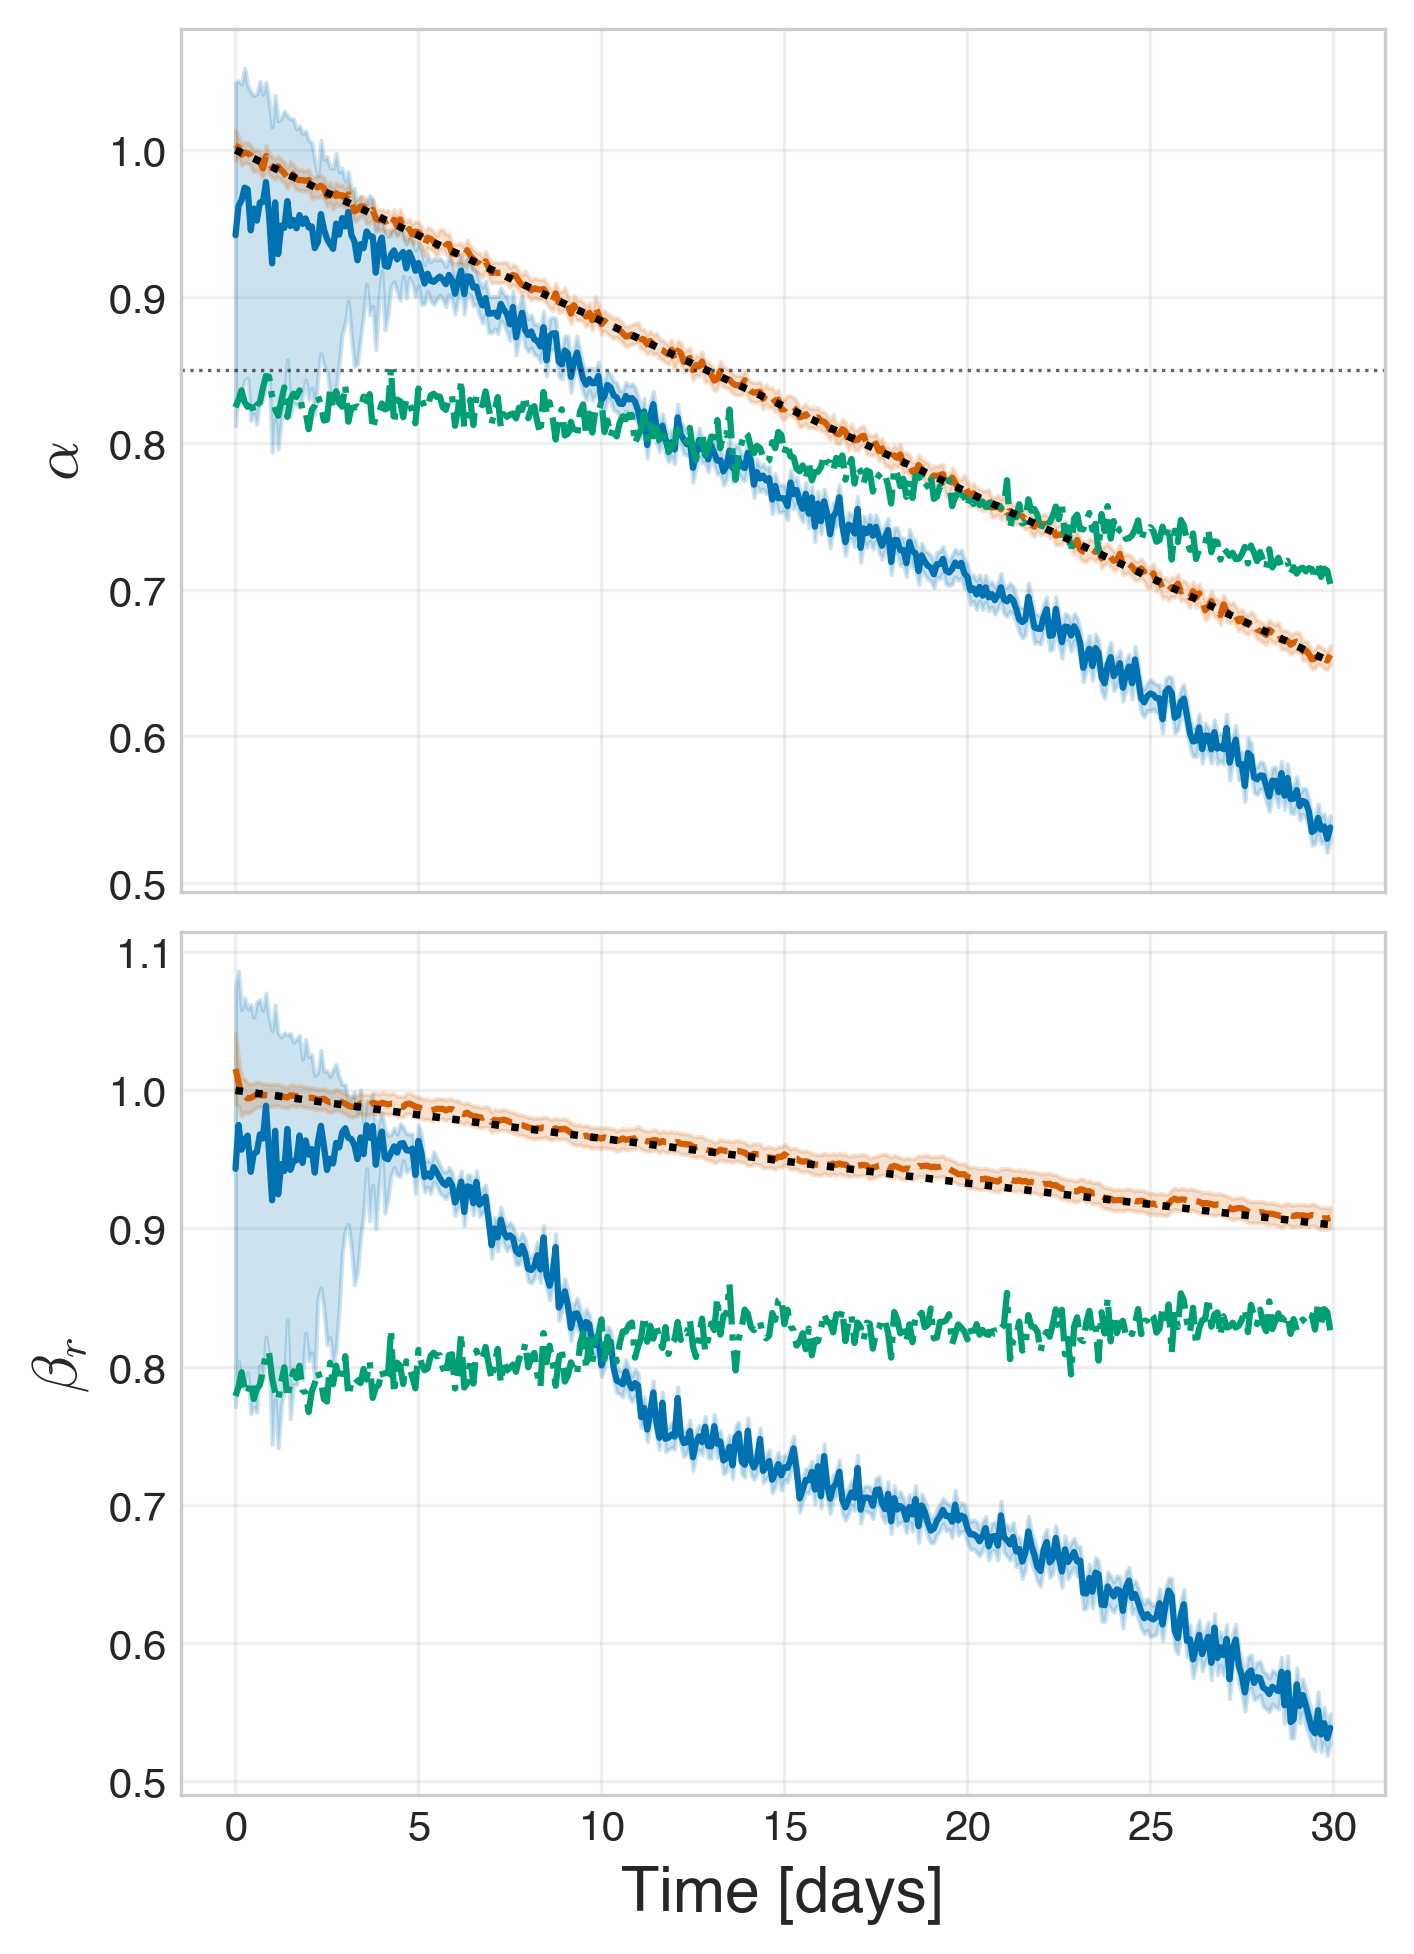
\includegraphics[width=0.95\linewidth]{nb27_sequential_tracking}
  \caption{30-day sequential tracking of $\alpha(t)$ and $\beta_r(t)$: SBI
    (hand-crafted 66-D posterior, blue) vs.\ EKF (orange), with 90\% CI/interval
    bands. True degradation profiles in black. The EKF tracks both parameters
    closely throughout; the SBI posterior mean diverges progressively from the
    true curve, most visibly for $\beta_r$, consistent with the reported MAE.}
  \label{fig:si_wu_sequential}
\end{figure*}
% ------------------------------------------------------------------

\subsection*{S11.3 Why the EKF wins here: control experiments}

Two competing explanations were tested and ruled out or confirmed in turn.

\textit{Control 1 -- same-shape trajectories.} Giving $\alpha$ and $\beta_r$
the same linear decay shape (removing any distinguishing temporal signature
between them) leaves the EKF's accuracy unchanged from the baseline result.

\textit{Control 2 -- static truth.} Holding both parameters fixed at the exact
W11 point ($\alpha=\beta_r=0.80$) for all 360 windows, the EKF converges to
near-perfect accuracy already in the \emph{first} window, not gradually over
the run. Together, Controls~1--2 rule out ``the EKF exploits sequential
structure that SBI's memoryless per-window treatment cannot'' as the
explanation: there is no evidence of information accumulating across windows
at all.

\textit{Control 3 -- EKF tuning.} An earlier EKF configuration (nb26) used an
overly tight initial parameter covariance and reported 0\% coverage at the
same $(\alpha,\beta_r)=(0.80,0.80)$ point this tracking run passes through.
Swapping in this notebook's more diffuse tuning on the \emph{identical} data
recovers both parameters to within $\sim$0.3\% error --- tuning alone flips
the outcome.

\textit{Control 4 -- robustness.} The diffuse-tuning result is not a lucky
draw: it reproduces across 15+ independent noise seeds at the W11 point and 4
additional $(\alpha,\beta_r)$ truth points spanning the identifiability-scan
grid.

\textit{Conclusion.} The EKF's advantage comes from privileged, exact-model
access to the raw, unaggregated 120-step trajectory at every window, not from
recursive/sequential structure --- the same mechanism identified independently
via the raw-trajectory FIM (the Artifact~2 discussion in the main text). A
trained CNN-embedding SBI posterior given the same raw-trajectory access
(Section~S10) narrows the $\beta_r$ gap (MAE $0.198 \to 0.139$) but widens the
$\alpha$ gap (MAE $0.048 \to 0.067$); neither closes the gap to the EKF, since
the EKF's advantage also includes exact-model (not merely raw-signal) access
that no amortised estimator receives.

% ---------------------------------------------------------------------------
\subsection{Limitations}
\label{sec:disc_limitations}
% ---------------------------------------------------------------------------

% ------------------------------------------------------------------
\begin{table}[htbp]
\centering
\caption{Limitations of the present study.}
\label{tab:limitations}
\small
\begin{tabular}{p{0.24\linewidth}p{0.68\linewidth}}
\toprule
Limitation & Note \\
\midrule
Synthetic data only &
  Both systems are evaluated on simulator-generated data; no real-plant
  validation or model-mismatch study is attempted here. \\
Structural bias is quantified, not eliminated &
  The $\beta$ (System~I) and $\alpha$/$\beta_r$ (System~II) offsets are
  characterised and shown to be representation-independent
  (Section~\ref{sec:disc_artefacts}), but recalibration requires scheduled
  open-loop excitation (Section~\ref{sec:disc_practical}), which was not
  deployed on a physical plant in this study. \\
SNPE seed instability &
  Training is seed-unstable at System~II's dimensionality; every
  System~II posterior reported in this paper required an 8-seed
  ensemble-and-select procedure rather than single-seed training. \\
Structure S-A calibration &
  0/40 tested seeds passed simulation-based calibration for Structure~S-A;
  this is a settled negative result, and no quantitative S-A claim is made
  anywhere in this paper. \\
QSS column-model stability &
  The quasi-steady-state column shortcut is numerically unstable below
  $\eta_\mathrm{col} = 0.80$; two candidate scenarios were excluded from
  the study on this basis. \\
No real-time deployment &
  Neither posterior was integrated with a live SCADA or process historian;
  the stateless, per-window design (Sections~\ref{sec:sequential_tracking},
  \ref{sec:wu_sequential}) is intended to make such integration
  straightforward, but it was not tested. \\
CNN-embedding architecture search &
  The architecture-sensitivity documented for the hand-crafted pipeline
  (larger networks did not improve, and sometimes worsened, System~II
  performance) transfers to the embedding-net variant; the modest CNN
  budget used here (Section~\ref{sec:disc_artefacts}) leaves open whether
  a larger search would resolve Artifact~2. \\
\bottomrule
\end{tabular}
\end{table}
% ------------------------------------------------------------------


\bibliography{references}

\end{document}
